\documentclass[a4paper, 12pt]{jsreport}
\usepackage{sisthesis}
\usepackage{bm}
%ここから上は変更しない

\title{振動刺激によるアリの行動変化の映像解析}

\author{ホアンバフン}
%提出年月
\submitdate{2024年1月}
%指導教員
\principaladviser{川嶋宏彰教授}
%入学年度
\enrollmentyear{2020}
%学籍番号
\studentid{JB20S079}

%表目次・図目次を表示したい場合はコメントアウトする
%\figurespagetrue
%\tablespagetrue


%使用するパッケージ
\usepackage[dvipdfmx]{graphicx}
\usepackage{tabularx}


\begin{document}

%beforeprefaceは必須
\beforepreface

\prefacesection{概要}
アリという生物は集団としてフェロモンを利用し行動することがよく知られている. フェロモンを利用するならばフェロモン信号を確認しながら行動するので移動速度がそれほど大きくないという特徴がある. 一方, 外から刺激が与えられた時にはいつもより早い速度で逃げていくアリが存在するのに対して, ほとんど動かず刺激の影響を受けないようなアリも存在する. また, 逃げるアリの中には巣に向かって逃げていくアリが多くみられる. そこで, 本研究では, 刺激が与えられた時の軌跡データに基づくアリの行動解析手法を提案する. 本提案手法の目的は, 刺激が与えられた時のアリの行動変化を明らかにすることである. 本研究では, 実際に刺激を与えてアリの行動変化誘発実験を行い, その様子を映像で記録する. この観察実験で得られる映像を用いてアリの個体群を追跡する. 追跡手法は物体検出手法であるYOLOv5と追跡( フレーム間対応付け)手法であるStrongSORTを組み合わせて利用する. 学習用データセットはアリの画像を手動でアノテーションして作成する. ただし, 追跡手法の精度には限界があり, 欠陥するデータの存在するため追跡結果データの前処理する必要がある. 処理したデータを軌跡データとしてアリの行動変化を解析する. 解析結果より, 以下のことが明らかになった. (1) 刺激を与えられるとアリ集団の速度が上昇する傾向が見られるが, 上昇する期間が短くまた元の速度で動く. (2) 同じ刺激を与えられてもよく動くアリと動かないアリがいる. (3) 動かないアリの方は速度上昇期間は短く, 実験に用いた板の中心部(餌の近辺), またはコロニーの近くにいることが多い.(4) よく動くアリの方は速度上昇期間が長く, 移動軌跡としてはコロニーに戻る傾向が見られる.より多くのデータ解析から, これらの知見の信頼性を上げることが今後の課題となる. 
%afterprefaceは必須
\afterpreface
\chapter{序論}

\section{研究背景}
\label{sec:background}

アリは個々の個体が独立に動くだけでなく, フェロモンを用いるコミュニケーションや接触などによる直接的コミュニケーションを用いて他個体と相互作用することがよく知られている\cite{1}. そして, 個々のアリが餌を発見して, その餌を巣 (コロニー)に持ち帰る行動などは集団全体に影響を与えることが明らかにされている~\cite{2}. 

また, アリはさまざまな環境条件下で生息しており, 外部からの刺激を受けることが多く, この外部からの刺激に対する適応能力が求められる. 外部刺激の一つとして, 振動刺激はアリのコミュニケーション(情報伝達)や探索及び帰巣行動に影響を与えることがある~\cite{3}. 一方で, 実際のデータに基づく詳細な分析はこれまで十分になされていない.

ここで, 近年は生物の移動をリアルタイムで高精細に観察し把握する映像技術が発達してきている~\cite{4}. これにより, 様々な生物について行動パターンや反応を詳細かつ客観的に分析することが可能になる. 

こうした映像解析技術を用いて振動刺激によりアリの行動解析ができないだろうか. 
\section{関連研究}
\label{sec:thesis}
アリの行動の観察や解析についての研究がされている. 
\paragraph{少数の働きアリによる行動解析とモデル化}~\cite{5}

これは障害物がない閉空間に少数の働きアリを放ち, 行動を観察計測しアリのコロニーにおける情報交換を推定していく研究である. 画像処理方法は既存ツールを用いており, 動画から一定間隔で静止画像を切り出したうえで, アリの移動距離をLabView+Ni Visionというソフトウェアで算出する. 解析結果より, アリの移動速度は一定ではなく変化していくことが明らかにされている. また, 速度変化していない状態が繰り返すアリが存在することも示されている. さらに, アリの各個体が移動と一休止を繰り返していることも見出されている. 「動く」と「休む」が交互に繰り返されていることから, アリは個体に特有の行動リズムを持っていることやフェロモンを導入することで観測された行動特性をモデル化できることなどが考察されている. 
\paragraph{アリの行動観察とその統計解析}~\cite{6}

これはRadio Frequency Identification(RFID)を用いてクロオオアリを長時間観察する研究である. 餌箱と餌場の間に観測センサを設置し移動時間帯を記録している. アリコロニーの活発度合いを図る指標として活発回数が提案されており, 個体ごとに観測期間での総活発回数が算出されている. 結果として, 働く回数は個体によりかなりの差があり, 大半の労働が一部の個体に依存することが明らかにされている. 加えて, 活発量の相関係数を用いて個体同士がどのように一緒に働いているのかが定量化されている. 相関係数の変化を算出することで, コロニー内の相互作用が見えなくとも統計的にどのように協働性を保ちながら活動をしているかを推定しようとするアプローチである. この研究ではこれまで研究者の経験に依存していた考察をデータ解析を利用することでより厳密に実証することを可能にしている. 
\section{研究目的とアプローチ}
\label{sec:aim}
\begin{figure}[tbp]
\centering
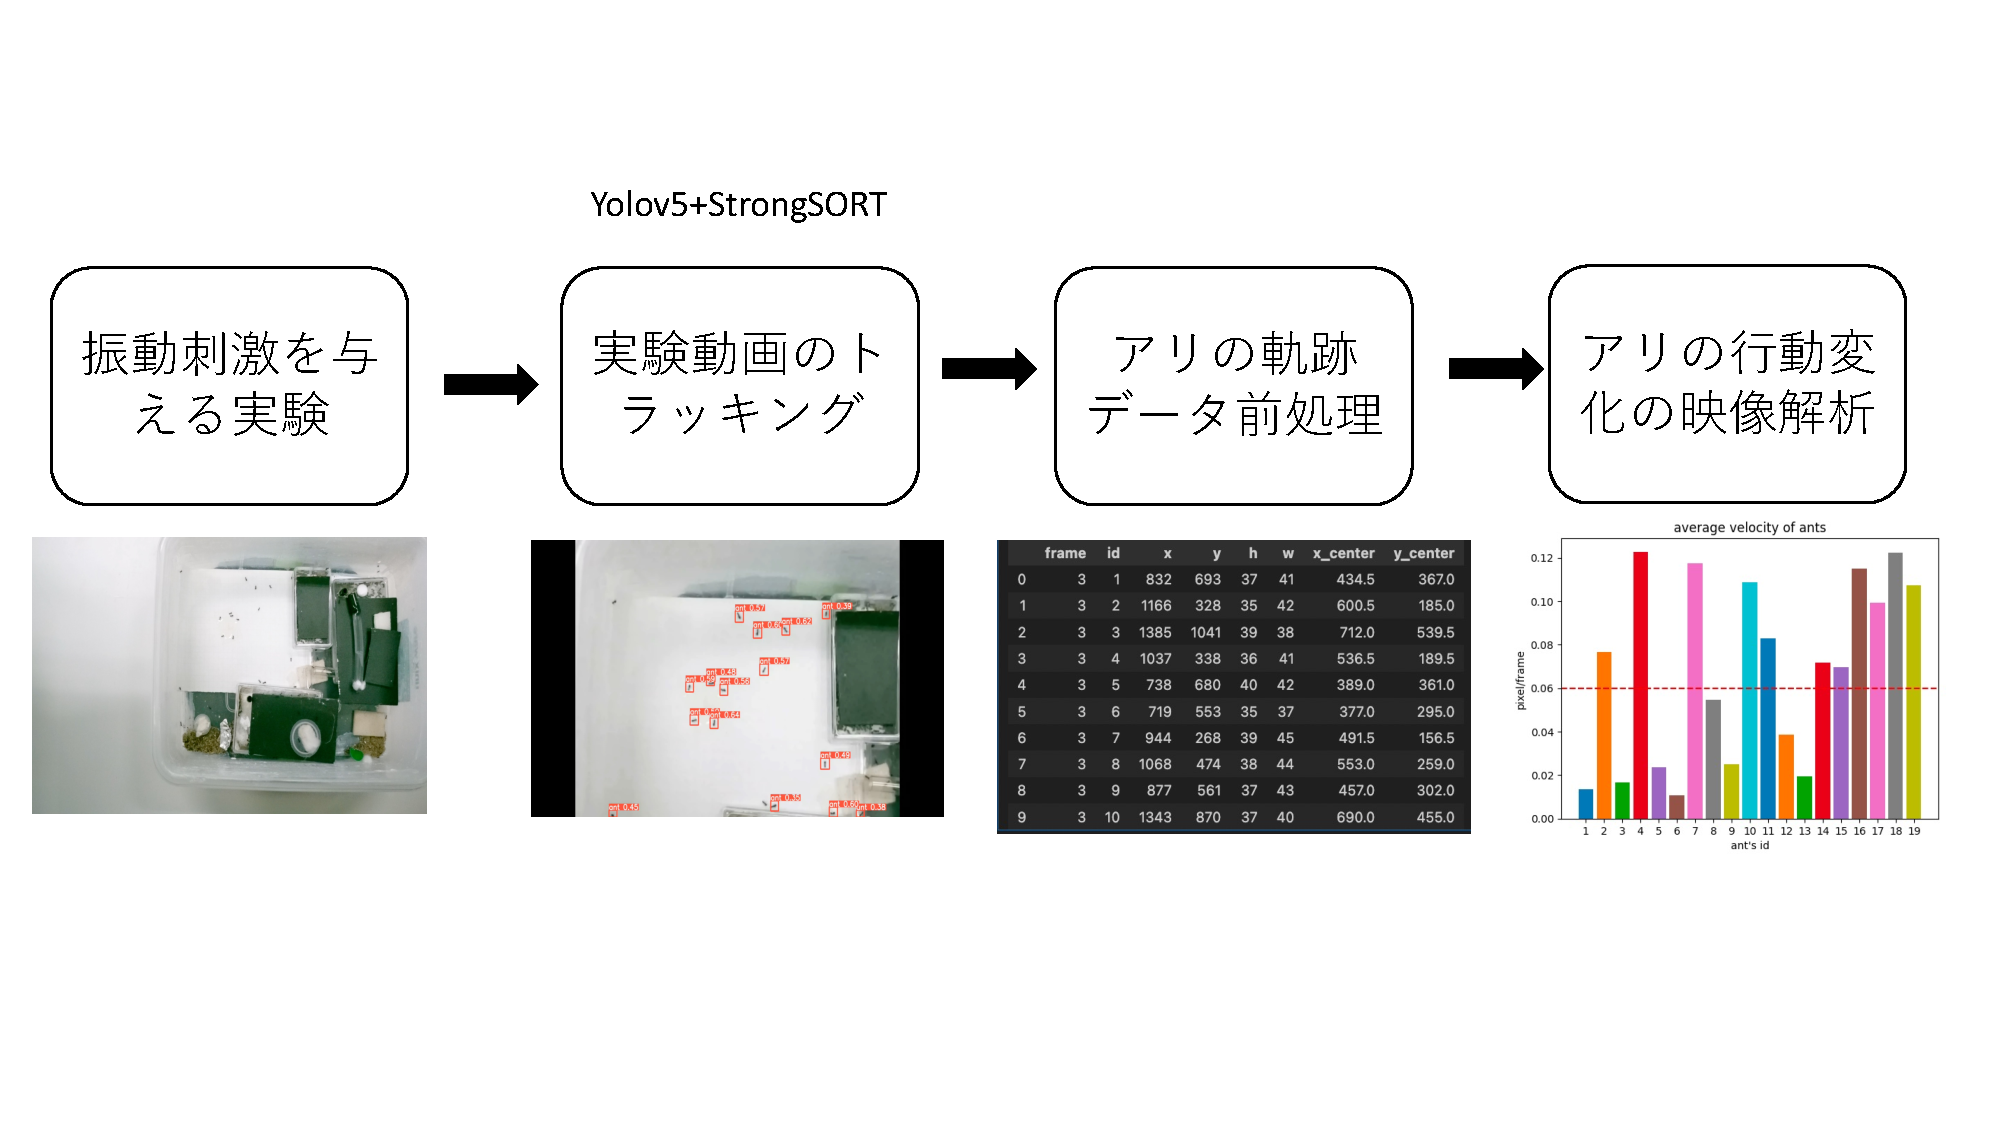
\includegraphics[width=13cm,  keepaspectratio]{nagare.pdf}
\caption[Short figure caption for List of Figures]{提案手法全体図}
\label{fig:paper1_fig1}
\end{figure}
\ref{sec:background}節で述べたように, 外部からの振動刺激の影響を映像解析によって定量的に測定することで, 行動変化を検出し, 理解することが期待できる. そこで本研究は, アリが振動刺激に対してどのように反応し, その行動パターンにどのような変化が生じるかを明らかにすることを目的とする. これにより, アリが環境刺激に対してどのように適応し, コミュニケーションや行動(帰巣・探索)にどのように影響されるかを理解することにつながる. 

本研究の流れを図1.1に示す. まず, 振動刺激の影響がアリの行動をどのように変化させるのか実験を行う. シミュレーションを用いる方法もあるが, シミュレーションはある程度まで既知の知見を元に構築したモデルを用いて行われるため, 未知の要因や予測できない事象に十分対応できない可能性がある. 一方で, 実際に実験で得られるデータを解析すれば未知の要因や新しいパターンを発見することができる. 次に, 実験動画でアリを追跡する. 関連研究ではRFIDを利用してアリの位置情報や移動距離など把握することができる. しかし, RFIDはあらかじめ設置した読み取りゾーンでしか個体を検出できず, 2次元的な広がりを持つパターンの解析には不向きであるので, 本研究はこれを利用することが難しいと判断して物体追跡手法を利用する. 追跡手法は個体検出手法であるYOLOv5とフレーム間でのIDの対応付け手法であるStrongSORTの組み合わせを利用する. 追跡した結果, それぞれのフレームにいるアリの位置情報を得ることができる. 追跡結果の軌跡データより, 刺激提示前後のアリの速度変化を全個体及び各個体別で解析し, アリの行動が振動刺激により個体レベルと集団レベルでどのように変化するかを説明する. 



\section{本論文構成}
\label{sec:struc}
本論文は全5章で構成されている. 序論に続き, \ref{chap:exp}章では振動刺激提示によるアリの行動変化誘発実験について述べる. \ref{chap:trac}章ではアリの個体群の追跡手法を述べる. 続いて, \ref{chap:analys}章では軌跡データを用いたアリの行動解析を, 5章では結論をそれぞれ述べる. 
\chapter{振動刺激提示によるアリの行動変化誘発実験}
\label{chap:exp}
本章では振動刺激によってアリの行動変化を誘発する実験について述べる. \ref{sec:expaim}節では実験の目的を述べ, \ref{sec:method}節では実験する方法を述べる. 続いて, \ref{sec:look}節において実験の注意点と困難性を説明し, 最後\ref{sec:expresult}では実験結果を述べる. 
なお, 本実験を行うために, 明治大学・西森研究室 研究員久本峻平氏に手順や方法を教えて頂いた. さらに, 久本氏には現場に来てアリの実験の適地を見つけていただくとともにサンプル実験をして頂いた. 
\section{実験目的}
\label{sec:expaim}
本研究の実験では比較的に集団で行動することの多いトビイロケアリ (以下では単にアリ) を実験に用いる. 
実験の目的は人為的に外部から振動を起こすことにより刺激を与え, アリの行動の変化を誘発させて, その行動変化を観察して録画し解析データとして保存することである. 
具体的な手順としては, まず決まった場所に餌を与えてアリが集まってくるまで待つ. 10匹以上のアリが集まってきたら刺激を与えてアリの行動変化を起こす動画を撮り保存する. 
\section{実験方法}
\label{sec:method}
実験は兵庫県立大学で行う. 明治大学・西森研究室研究員久本氏の協力により実験を実施した. 実験に用いる器材等を図2.1及び図2.2に示す. 



\begin{figure}[tbp]
\centering
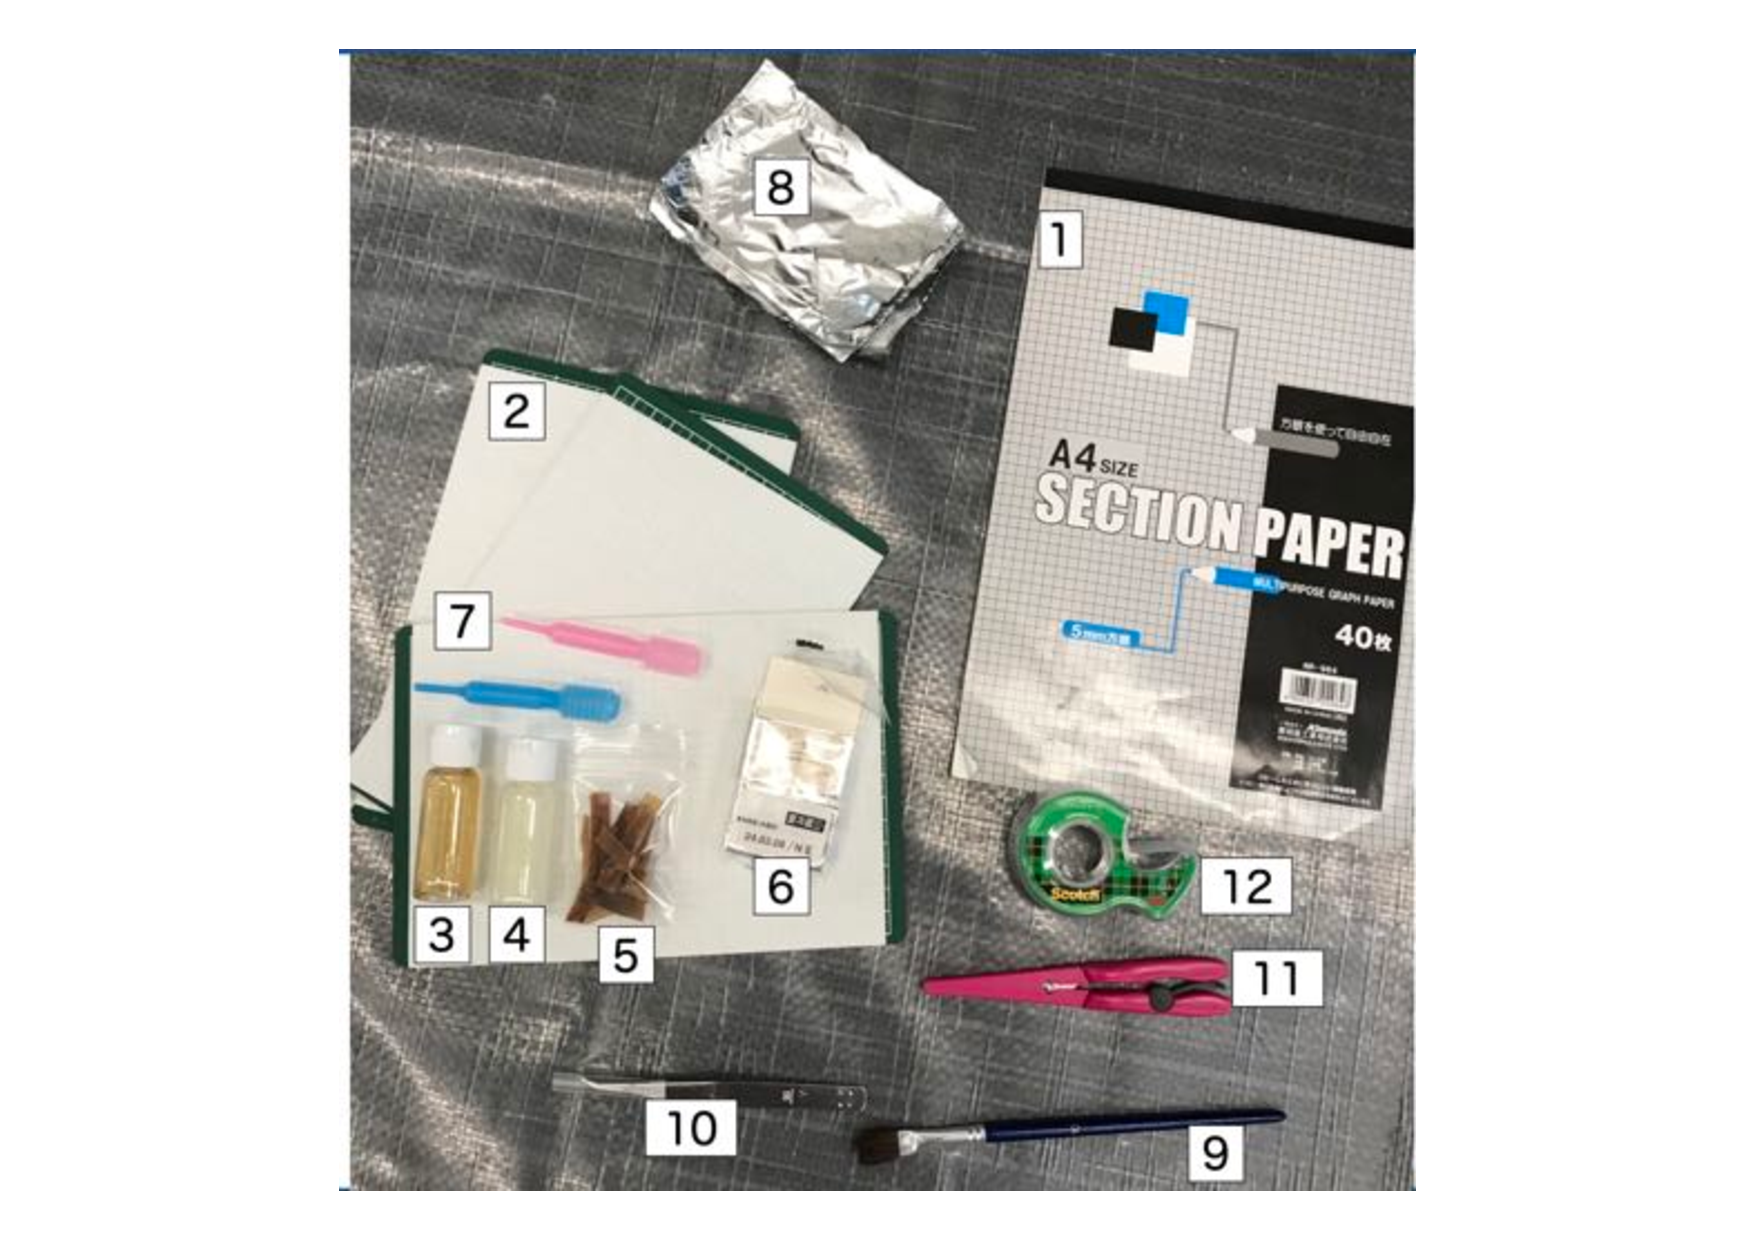
\includegraphics[width=13cm,  keepaspectratio]{exp1.pdf}
\caption[Short figure caption for List of Figures]{野外実験用の物品}
\label{fig:paper1_fig2}
\end{figure}
\begin{figure}[tbp]
\centering
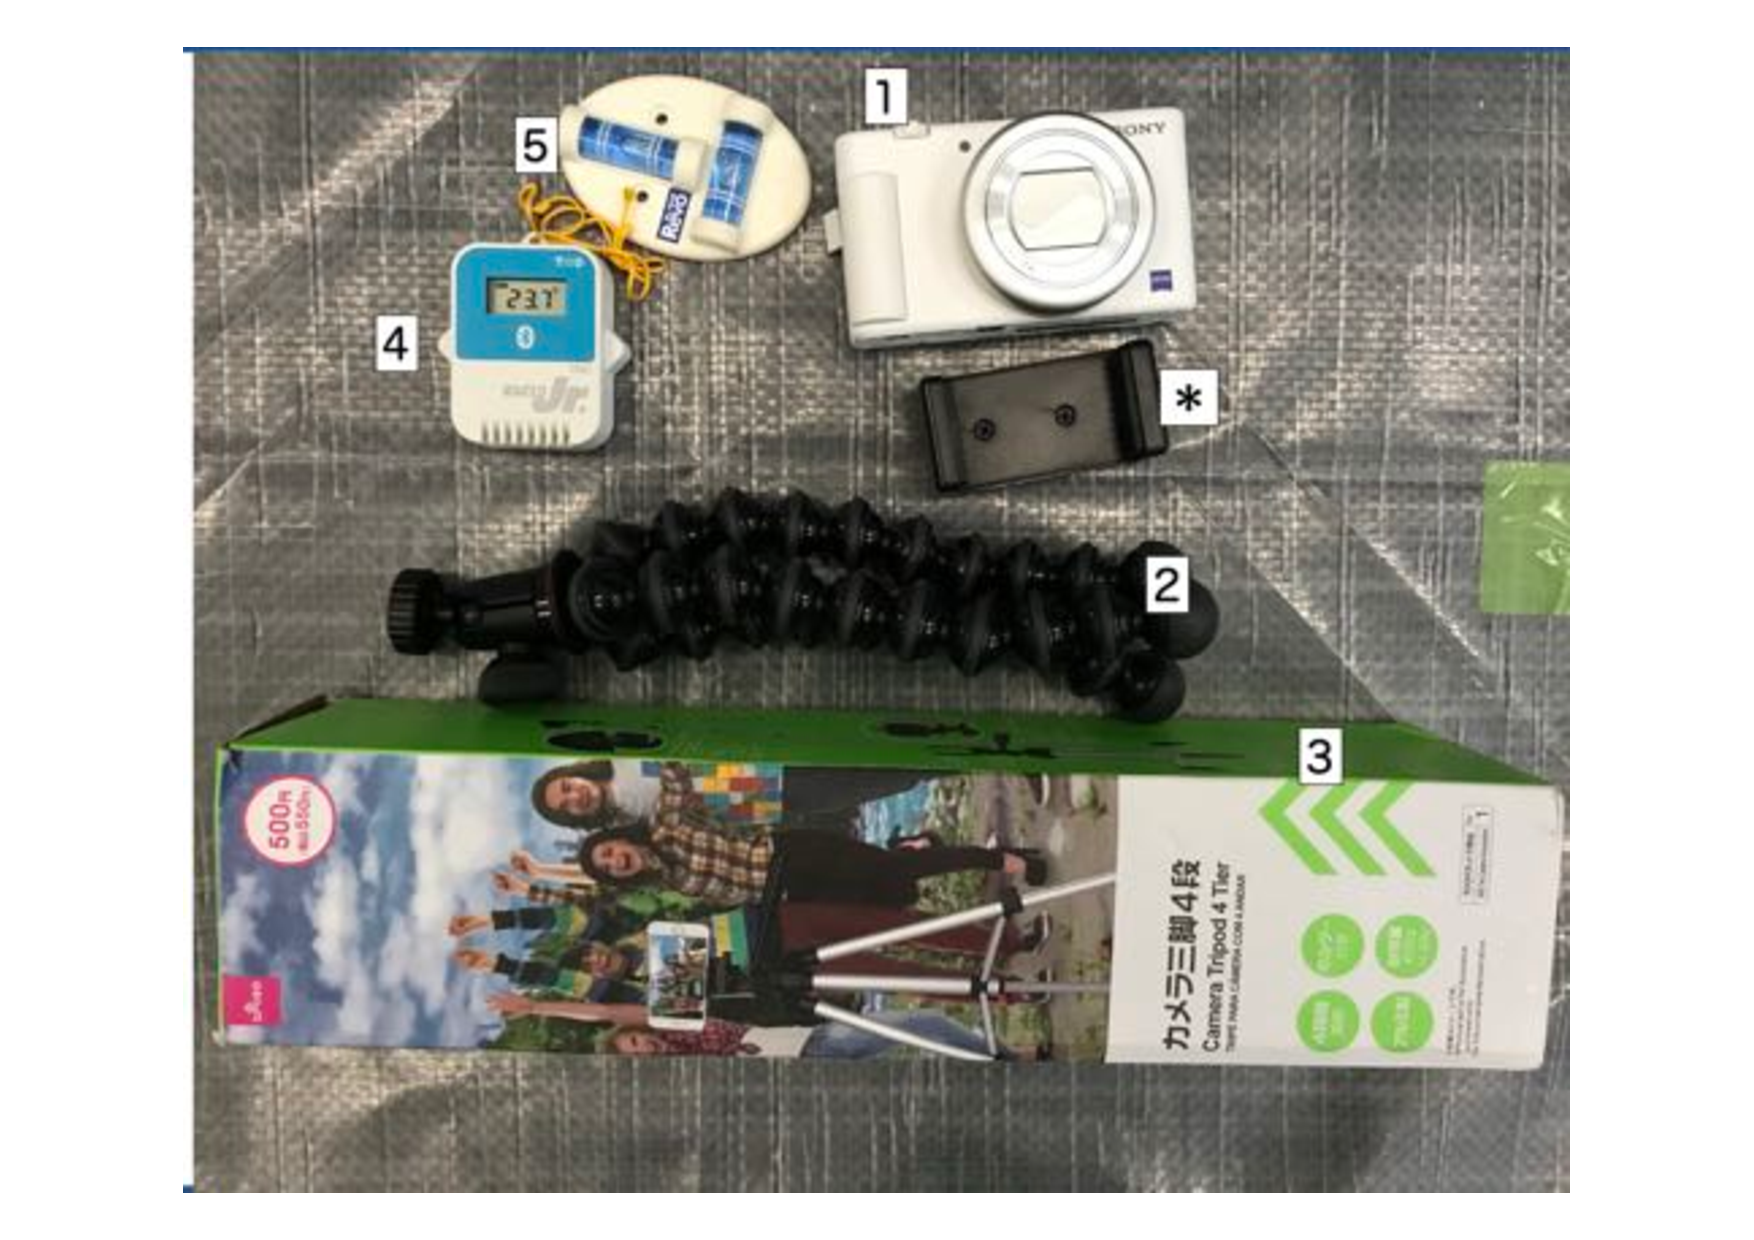
\includegraphics[width=13cm,  keepaspectratio]{exp2.pdf}
\caption[Short figure caption for List of Figures]{撮影系物品}
\label{fig:paper1_fig3}
\end{figure}
\paragraph{野外実験用の物品}
図2.1はアリの誘引や観察環境を設けるために用いており, 具体的には以下の物品である. 
\begin{enumerate}
   \item 方眼紙:背景の調整 スケール用 実験ごとに剥がして交換
   \item カット板:方眼紙を貼り付け, サイズは状況に合わせて
   \item ハチミツ(希釈):蜜系エサ
   \item カルピス原液:蜜系エサ
   \item スルメジャーキー:固形エサ
   \item ベビーチーズ:固形エサ
   \item スポイト:蜜系エサの量を調
   \item アルミホイル:エサ置き
   \item 筆:アリをはらう
   \item ピンセット
   \item ハサミ(携帯用)
   \item テープ
 \end{enumerate}
\paragraph{撮影系物品}
図2.2は撮影を目的とするものであり, 以下の物品を用いる.
\begin{enumerate}
   \item カメラ(iPhone)
   \item ミニ三脚(自由に曲がるタイプ)
   \item 500円三脚(100均で売っているもの)
   \item 水平器
 \end{enumerate}

\paragraph{実験手順}
具体的な実験手順は以下の通りである.
\begin{enumerate}
   \item トビイロケアリを探す(木の幹)
   \item トレイルを追いかけて巣穴を探す→ここまでは久本さんが事前に見つけておく 
   \item  巣穴近くに方眼紙を貼り付けたカット板を置く
   \item カット板が水平かチェック
   \item 三脚, カメラをセット(場合によっては日傘をセット)
   \item 撮影開始
   \item カット板の上をアリが歩いているなら8へ歩いていないなら7(a)へ
   \begin{enumerate}
     \item 固形エサ(スルメジャーキーorチーズ)を巣穴付近に設置して誘引  
     \item 固形エサにアリが接触したら固形エサを巣穴から少し離す
     \item 固形エサからアリが離れて巣に戻ったら固形エサと巣穴の間にプラ板を置き蜜エサをホイルの上に垂らす
    \end{enumerate}
   \item ホイル片を置き蜜エサをホイルの上に垂らす
   \item 狙った数のアリが集まるまで待つ
   \item カット板にピンセットで叩くなどの衝撃を加える
   \item パニックになって巣穴に帰る
   \item 撮影終了
 \end{enumerate}





\section{実験の注意点と困難性}
\label{sec:look}
野外実験する時, 実験者の安全を確保しながら実験を適切に遂行するために注意することがある. 以下では, 実験に終k流注意点, および実際に実験を行った結果から得られる知見をまとめる. 
\begin{itemize}
   \item 実験時間帯
   \begin{itemize}
     \item 7月-8月は少なくとも11:00から18:00で可能である
     \item 暑い日は16:00から18:00の間に実験することを推奨する
     \item 風邪が強い場合は実験器具が飛ぶこともあるので注意する必要がある
     \item 7月末は蚊は少なかった. 8月の方が多く出るが9月になるとほとんど出ない( 行動が非活性となる時期)
   \end{itemize}
   \item 実験に利用する餌
   \begin{itemize}
     \item 今回の実験に使ったのは「かの蜂 国産 百花蜂蜜」である. 安いハチミツは添加物があるので避けた方が無難である
     \item 7月末の実験では, 最も高い活性が得られた餌はハチミツ水(1/2希釈)である
     \item 風があるのでハチミツを使う場合はプラ板の上に乗せる方がいい
   \end{itemize}
 \end{itemize}
\paragraph{困難性}
野外実験の困難性はアリの活動時期があることである. 7月-8月末はアリの一番活動時期である. また, 活動時期といってもほとんど活動しない日があるし, アリが集まってくるまで時間がかかることがわかった. 


\section{実験結果}
\label{sec:expresult}
撮影実験を何度も繰り返した後に, 実験目的と合う動画を3本撮影できた. それぞれの実験では10匹以上のアリが集まってきてから振動を与えてアリの行動変化を起こした. 振動刺激の与え方を連続的( 複数回連続で繰り返す方法)にすることがしばしばアリの行動変化を誘発するのに必要であったが, 一方で, どの振動刺激がアリの行動に影響するかを解析することや刺激終了時刻の確定が難しくなり, 後段の解析が困難になることがわかった. 
\begin{figure}[tbp]
\centering
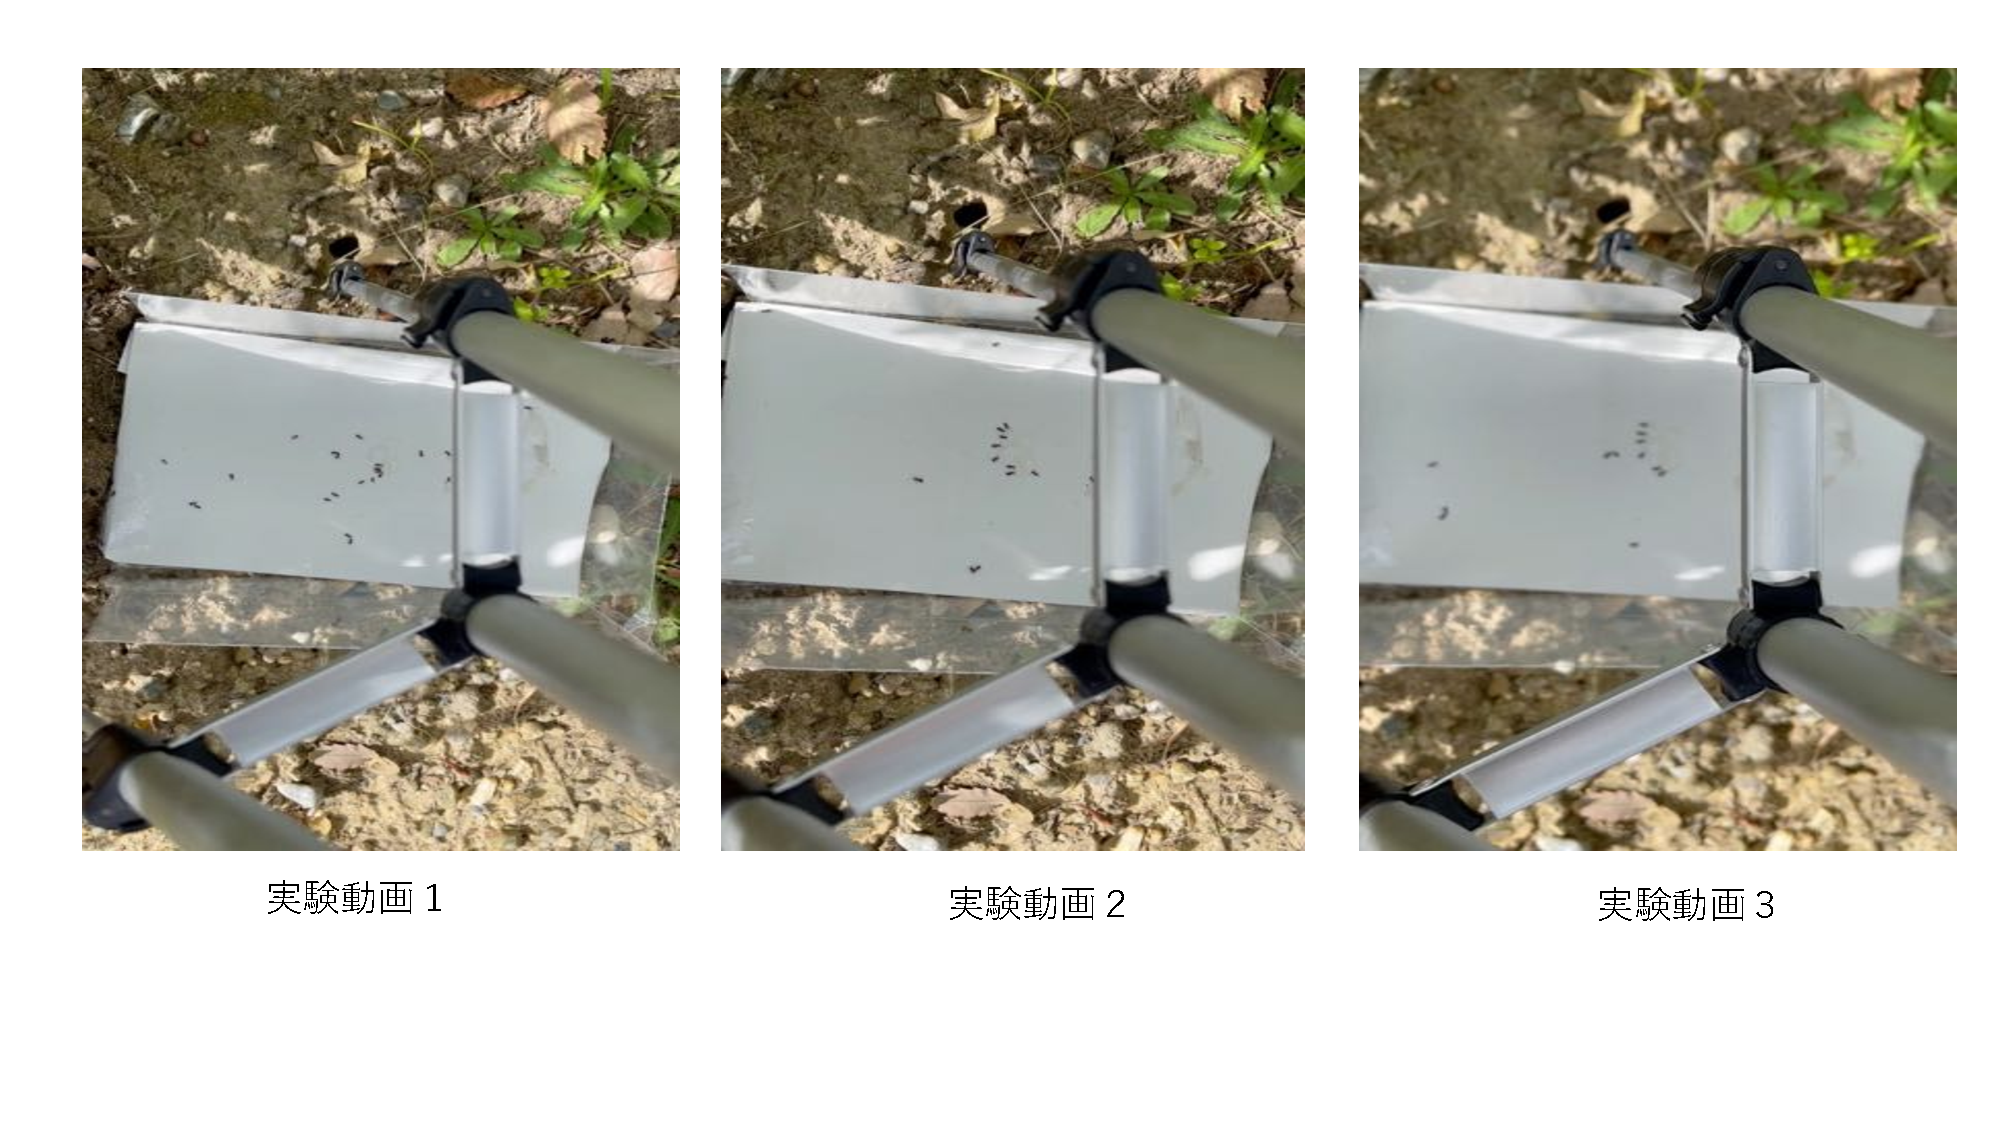
\includegraphics[width=13cm,  keepaspectratio]{exp_video.pdf}
\caption[Short figure caption for List of Figures]{野外実験動画}
\label{fig:paper1_fig4}
\end{figure}
\begin{figure}[tbp]
\centering
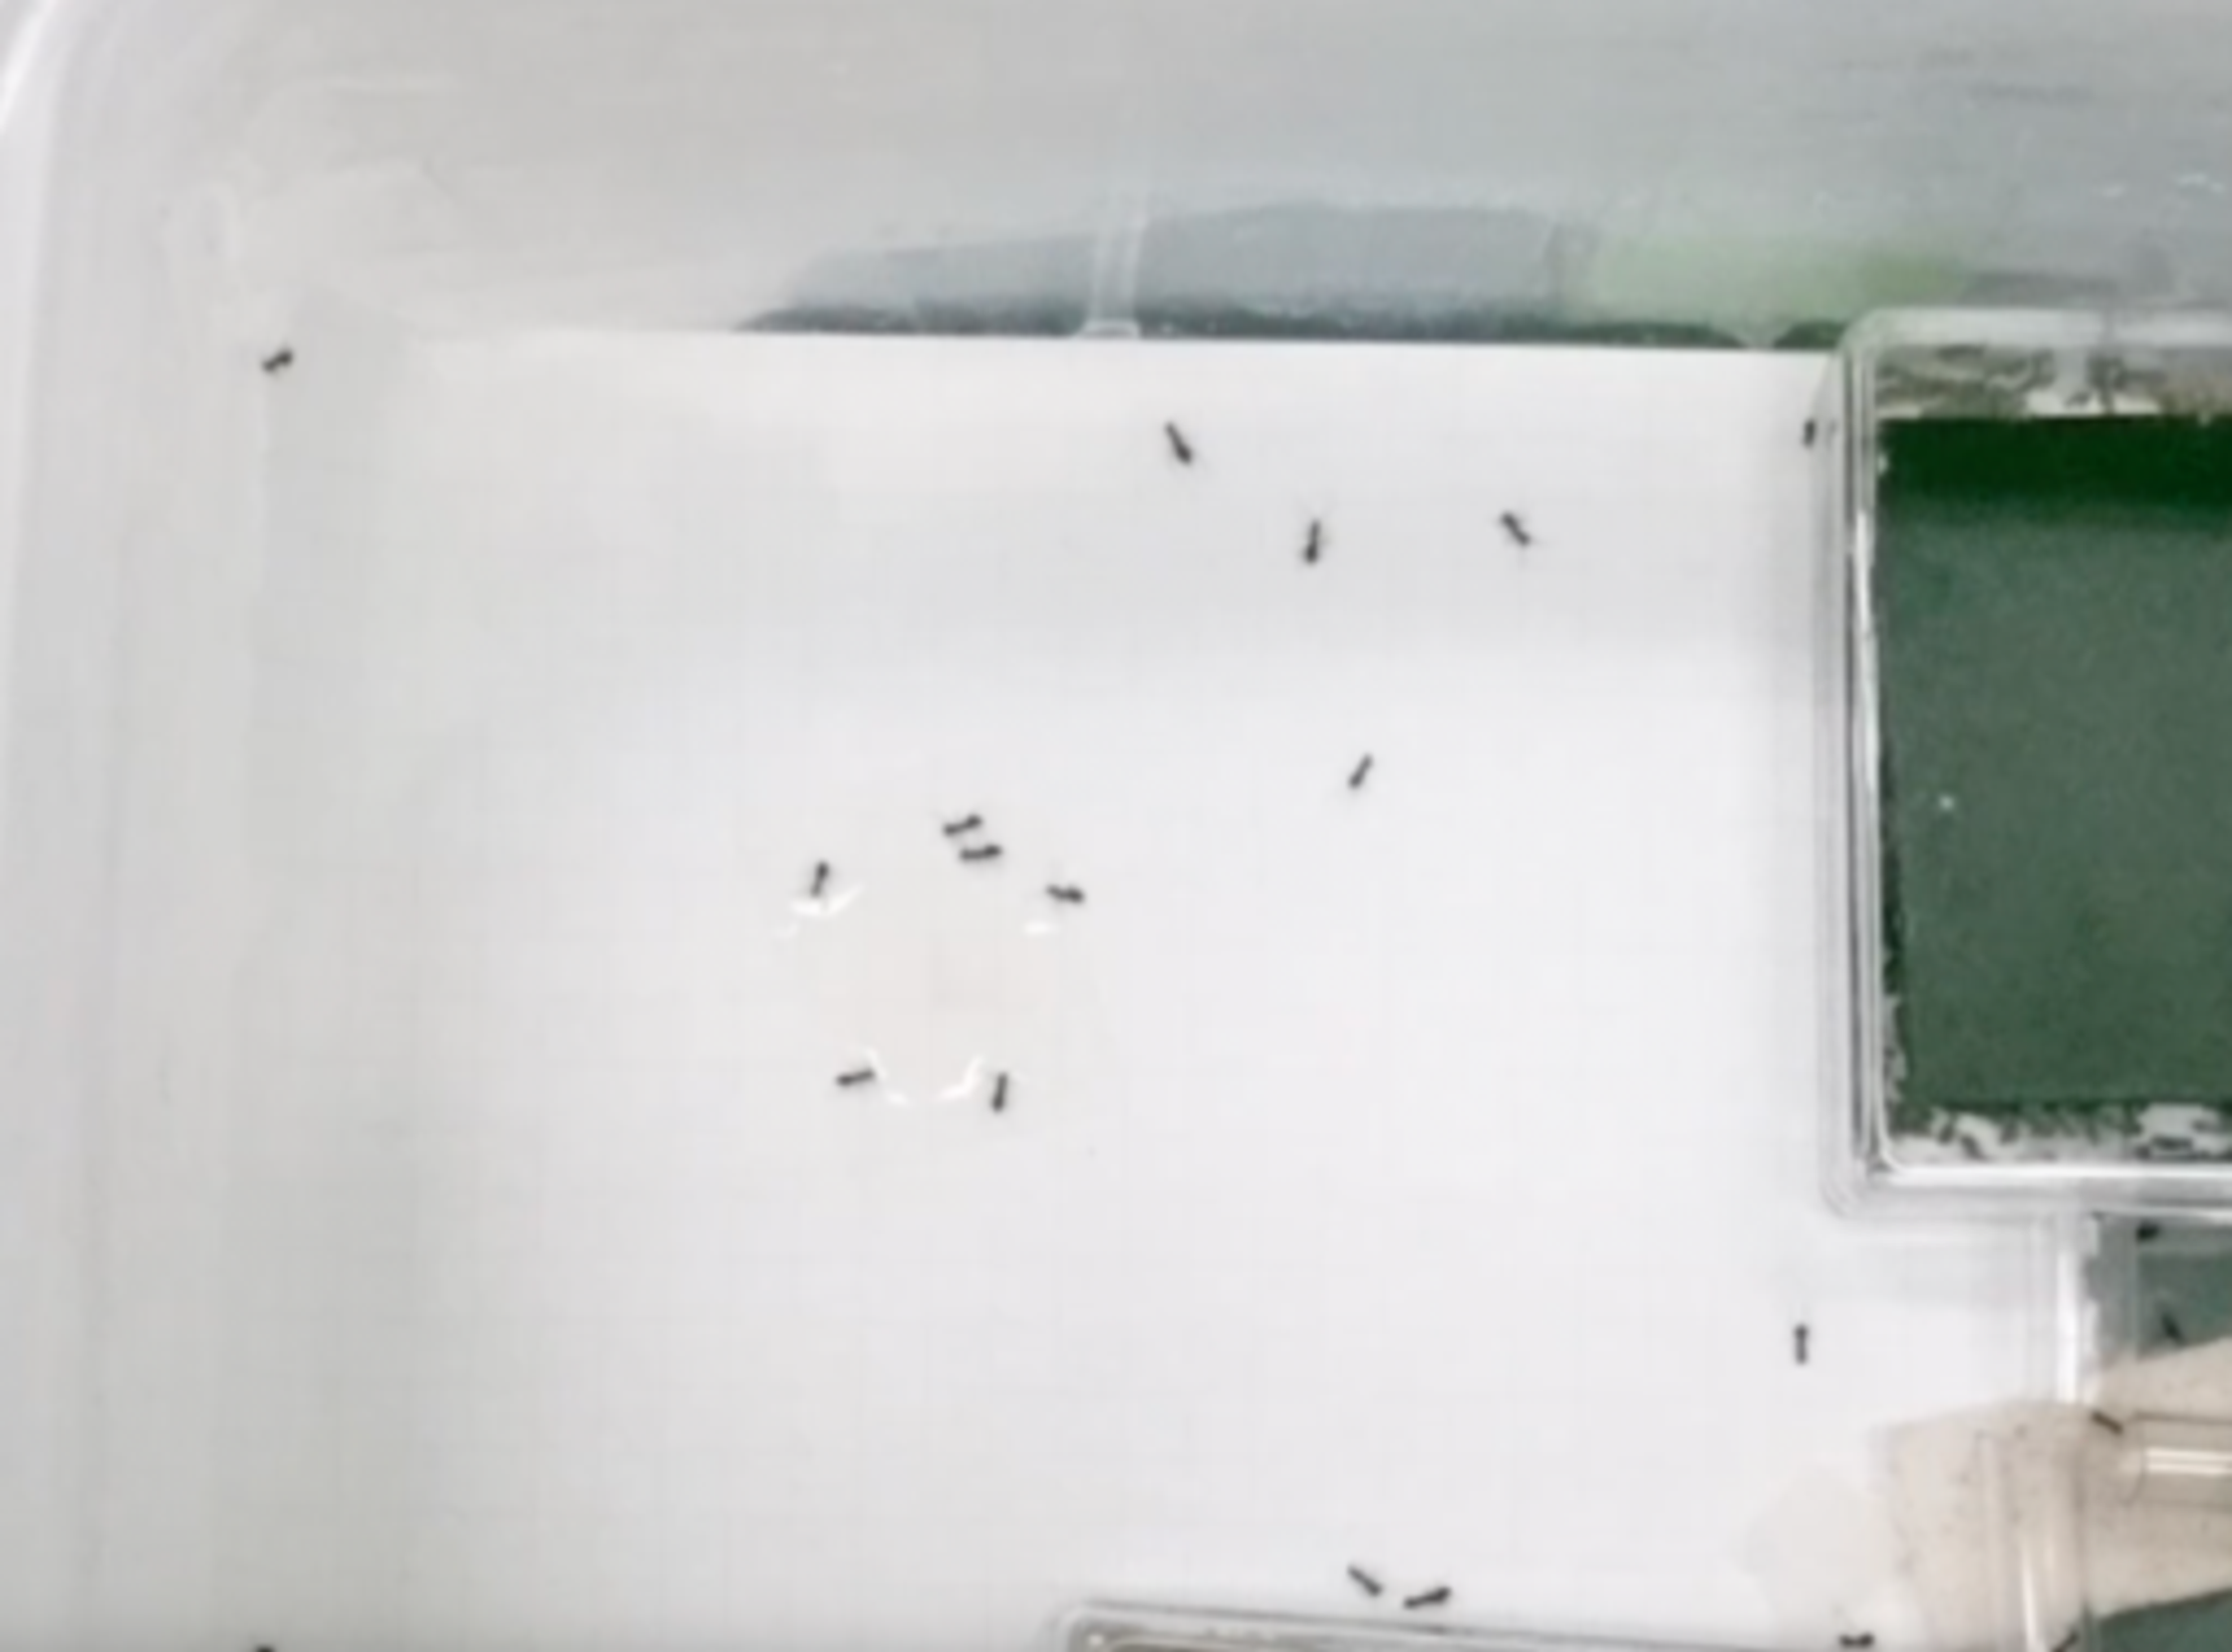
\includegraphics[width=13cm,  keepaspectratio]{exp_video_1.pdf}
\caption[Short figure caption for List of Figures]{研究室内実験動画}
\label{fig:paper1_fig5}
\end{figure}
野外実験と同時に研究室での実験も行った. これは明治大学の研究室内実験環境で実施され, そのデータの提供を受けた. 動画中の画像例を図2.4に示す. 室内のアリは, 野外アリとは異なり活発的な行動があまりみられなかった. しかし研究室での実験の特徴としては撮影条件の統制がとれることであり, アリの数も多いことで実験するのに適切である. 野外実験と同じ方法で餌を与えてアリが集まってくるのを待ち, その後に刺激を与える流れで行う. 

次章以降の解析では, 撮影条件の安定さを考慮して研究室での実験から得られた動画を用いるものとする. 具体的には, 1時間前後の長さの動画から刺激与える前5秒と後5秒の動画を切り取り解析データとして利用する. アリの数が少なく, 個体の動きがあまり被っていない動画において, 次章で述べる手法を用いて各個体を追跡する. 


\chapter{アリの個体群の追跡手法}
\label{chap:trac}
本章では第\ref{chap:exp}章で実現した実験動画を利用して追跡をする手法について述べる. 
まず, \ref{sec:detector}節において検出アルゴリズムと学習用画像データセット学習用データセット作成方法について述べる. \ref{sec:tracking}節では追跡アルゴリズムについて述べ, \ref{sec:result}節で追跡結果と追跡結果の考察を説明する. 
\section{検出アルゴリズムと学習用映像データセット}
\label{sec:detector}
検出アルゴリズム(物体検出アルゴリズム)とは画像を入力として画像内の位置情報を特定し, その物体位置情報を示すバウンディングボックス(bbox)を出力するとともにbboxに含まれる物体を識別する手法である. 近年提案されている多くの物体検出アルゴリズムはニューラルネットを用いている. 


複数物体検出アルゴリズムの中ではYOLOv5と呼ばれる手法の処理速度が非常に速く, リアルタイムに物体検出を行うことが可能という特徴を持ち, 検出制度も高いことから, 本研究ではYOLOv5を利用する. 

本研究ではアリを検出するので, アリのアノテーションデータセットを用意する必要がある. データセット作成用画像は実験と同じ種類のアリの別の動画を画像化し利用する. labelmeというアノテーションツールを使ってアノテーションデータセットを作成する. 今回作成した画像は231枚の中でランダムに学習用は183枚, 検証用48枚へ分割する. 作成したデータセットには画像データのほか, テキスト形式出保存されたアノテーションデータを含む. アノテーション情報のフォーマットは左からクラス(今回1クラスアリだけなので全て0になる), bboxの中心の座標$(x, y)$, bboxの横幅, 縦幅の順に記載される. 

手持ちデータセットは少ないので転移学習を用いて学習する. 転移学習とは一から学習する通常の学習と異なり, 学習済みのモデルを元に, 少ないデータでモデルを短時間で再学習する方法である. 学習時の指定オプションは, 学習済みモデルYOLOv5sに対して, バッチサイズ16に, エポック(Epochs)(50,  100,  200)に変更して学習した. 

結果を見ると50 epochsの時にはまだ学習余地があり, 200 epochsの時は習結果が横線で過学習になりがちであるので, 100epochsの時の学習が一番良いと判断した. 学習した重み(weight)を利用して, 実験動画を検出してみた. 
\begin{figure}[tbp]
\centering
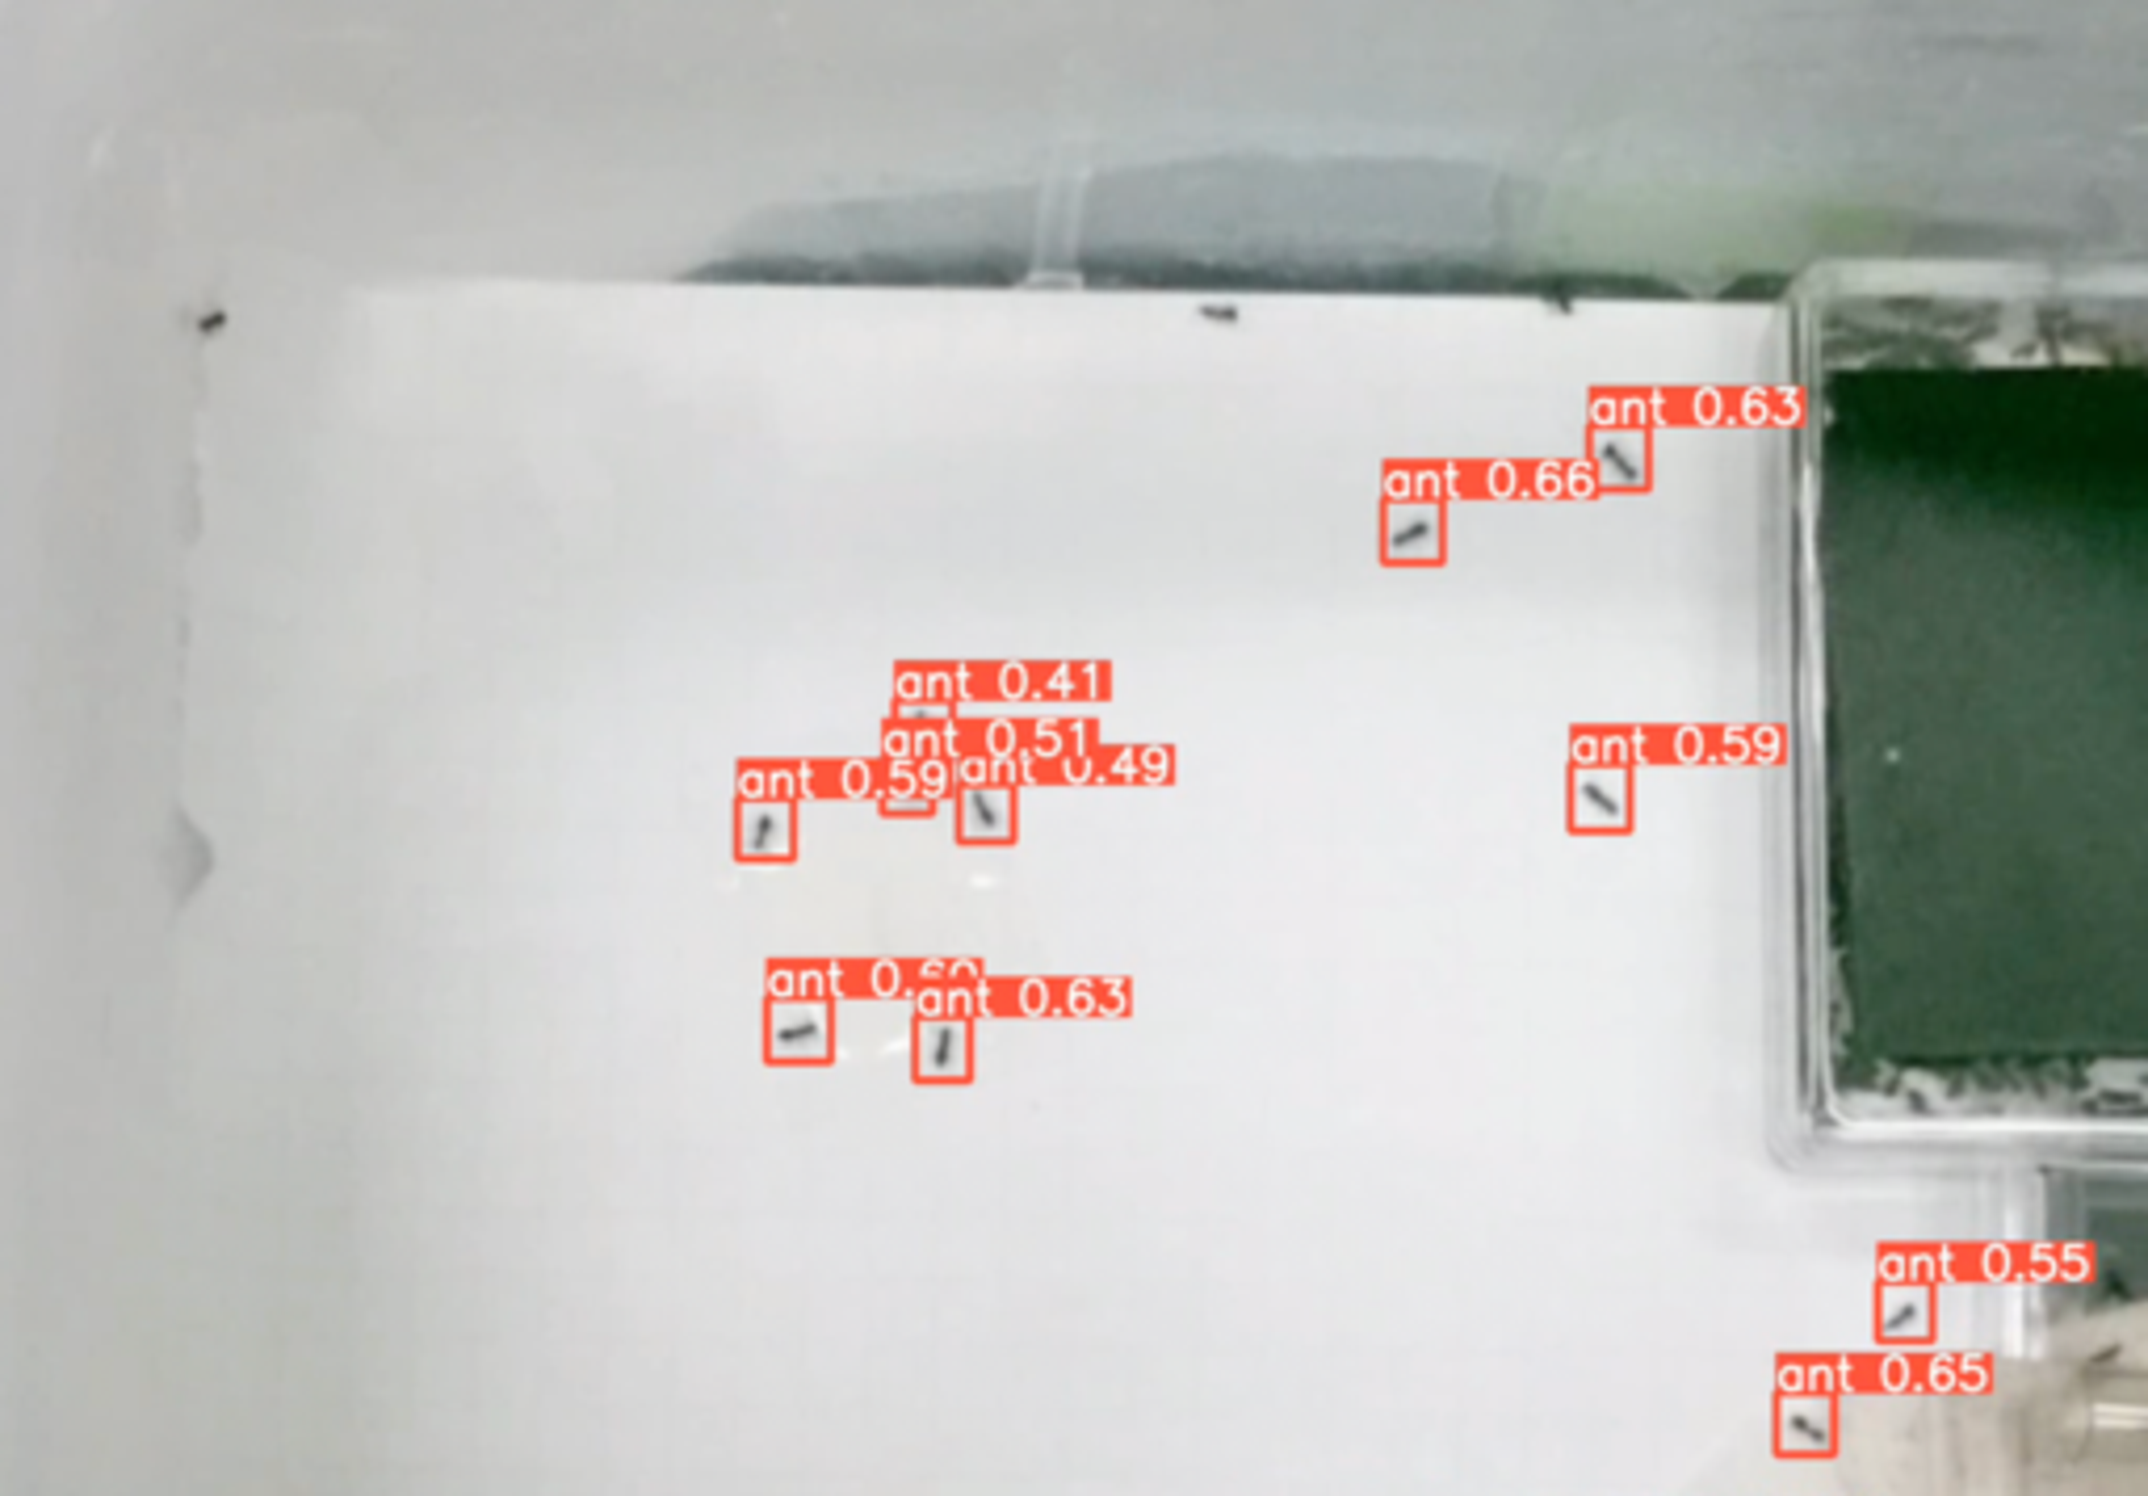
\includegraphics[width=13cm,  keepaspectratio]{detec.pdf}
\caption[Short figure caption for List of Figures]{検出結果}
\label{fig:paper1_fig6}
\end{figure}
小さくて形を判断しづらいアリは全て検出することは不可能であることがわかった. しかし, 多数のアリが検出できていることから, この結果を用いて追跡手法と組み合わせて追跡をする. 

\section{追跡アルゴリズム}
\label{sec:tracking}
生物追跡既存ツールとしてTRexとidtracker.aiなどの追跡ツールが利用されている. しかし, 本研究ではこれらのツールを利用しない. 理由としてはこれらの既存ツールは個体数が固定であることを仮定しているが, 本研究の実験では途中でアリの数が減ったり増えたりするので数を固定できないからである. 

コンピュータビジョンの分野で近年研究されている代表的追跡手法はSORT ( Simple and Online Realtime Tracking)~\cite{7}が挙げられる. この手法では, 物体検出器(たとえばYOLOv5などのDetector)によって取得されたbboxと, カルマンフィルタを使用して予測されたbboxのそれぞれの重なりをIoU(Intersection over Union)によって計算し, それをコスト行列とします. そして, コスト行列が最大となる検出物体と予測物体の組み合わせを, ハンガリアンアルゴリズムなどの組み合わせ最適化アルゴリズムを用いて探索し, 得られた組み合わせをフレーム間で関連付けていく. 

SORTの発展版としてDeepSORT(Simple and Online Realtime Tracking with a Deep Association Metric)~\cite{8}がある. DeepSORT手法はDetectorにより得られたbbox内の画像より畳み込みニューラルネットを利用して特徴抽出を行う. DeepSORTは誤検出を除去するのとトラッキングの不安定性を軽減するなどの特徴を持つ. 

StrongSORT~\cite{9}はDeepSORTをさらに発展させることで, 手法の提案時点では物体追跡ベンチマークにおける最高性能を達成したモデルである. StrongSORTはDeepSORTと同様に検出時と追跡時のモデルを別々に用意するものの, 外観特徴抽出器を改良するものを採用していることで精度向上を果たしている. 

本研究では追跡アルゴリズムとしてStrongSORTを用いる. 


\section{追跡結果と考察}
\label{sec:result}
検出器YOLOv5と追跡手法StrongSORTを利用してアリの動画の追跡を実施した. 
\begin{figure}[tbp]
\centering
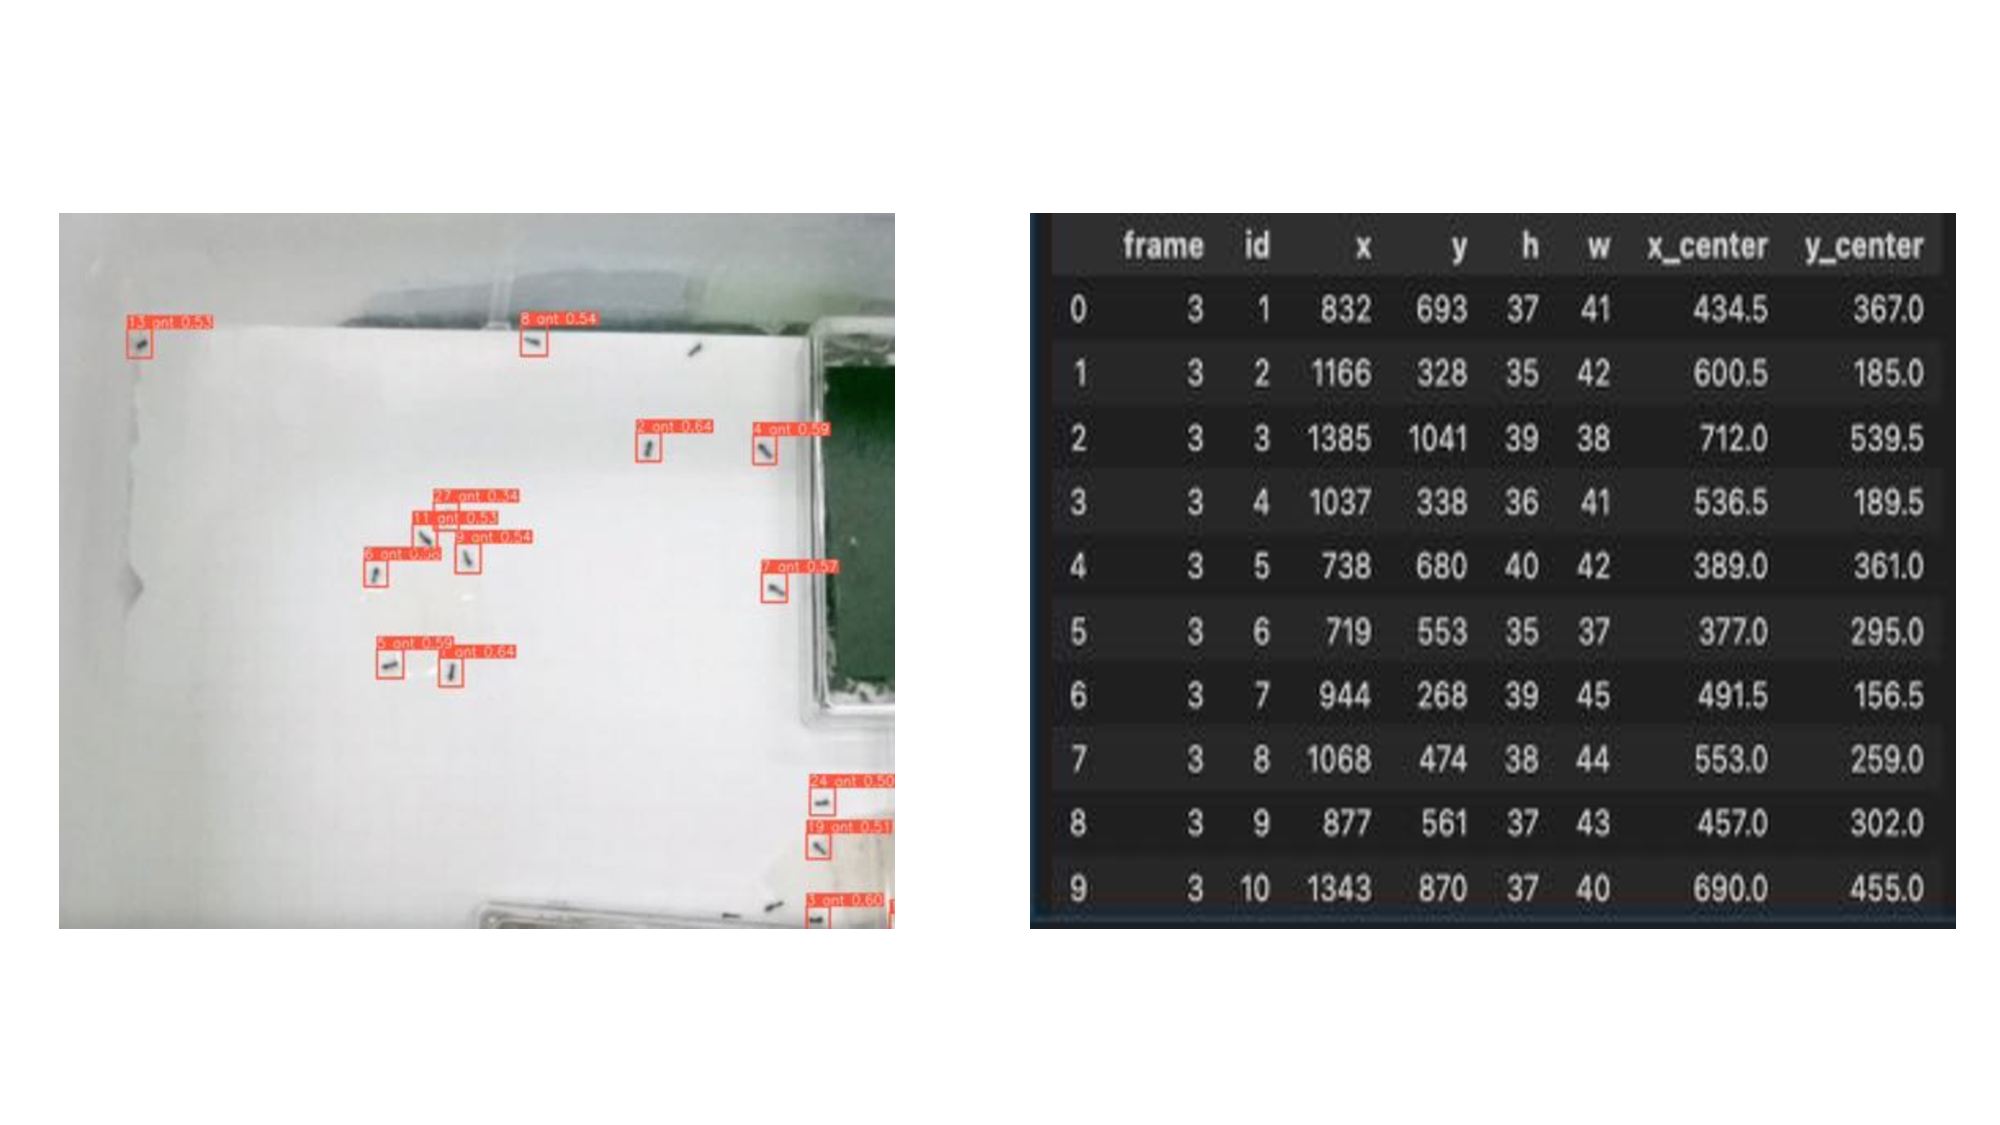
\includegraphics[width=13cm,  keepaspectratio]{tracking_data.pdf}
\caption[Short figure caption for List of Figures]{追跡結果}
\label{fig:paper1_fig7}
\end{figure}

追跡した結果は可視化用の動画と軌跡データのテキストファイルとして得られる( 図3.2). 可視化用の動画ではアリの位置とIDを確認することができる. 座標データファイルではそれぞれのフレーム, アリのID, アリの位置の情報を確認することができる. 

追跡手法の限界があるので完全に追跡できるのは不可能であることがわかった. 一度IDがつけられるが一時的に追跡できなった後に, また別のIDがつけられるアリがいる. 特に動く速度が速いアリの方でこの傾向がよく見られる. 
\chapter{軌跡データを用いたアリの行動解析}
\label{chap:analys}

本章では第\ref{chap:trac}章で追跡したデータを利用してアリの行動変化を解析する. まず, \ref{sec:process}節において軌跡データの前処理を行い, 信頼性の低いデータを削除する. 次に, \ref{sec:analys}節では振動刺激によりアリの集団における速度変化を解析し, それぞれのアリの行動の違いを解析する. 最後に\ref{sec:chiken}節において行動解析より得られた知見について述べる。
\section{軌跡データの前処理}
\label{sec:process}
追跡データからどのフレームにどのIDのアリが出現するかプロットした結果を図4.1に示す. この図の縦軸はフレーム番号, 横軸は個体のIDであり, セルに色が塗られている箇所が, そのフレームでそのIDの個体が出現したことを示す. これを見ると出現回数( 出現フレーム数)が比較的少ないアリがいる. 

\begin{figure}[tbp]
\centering
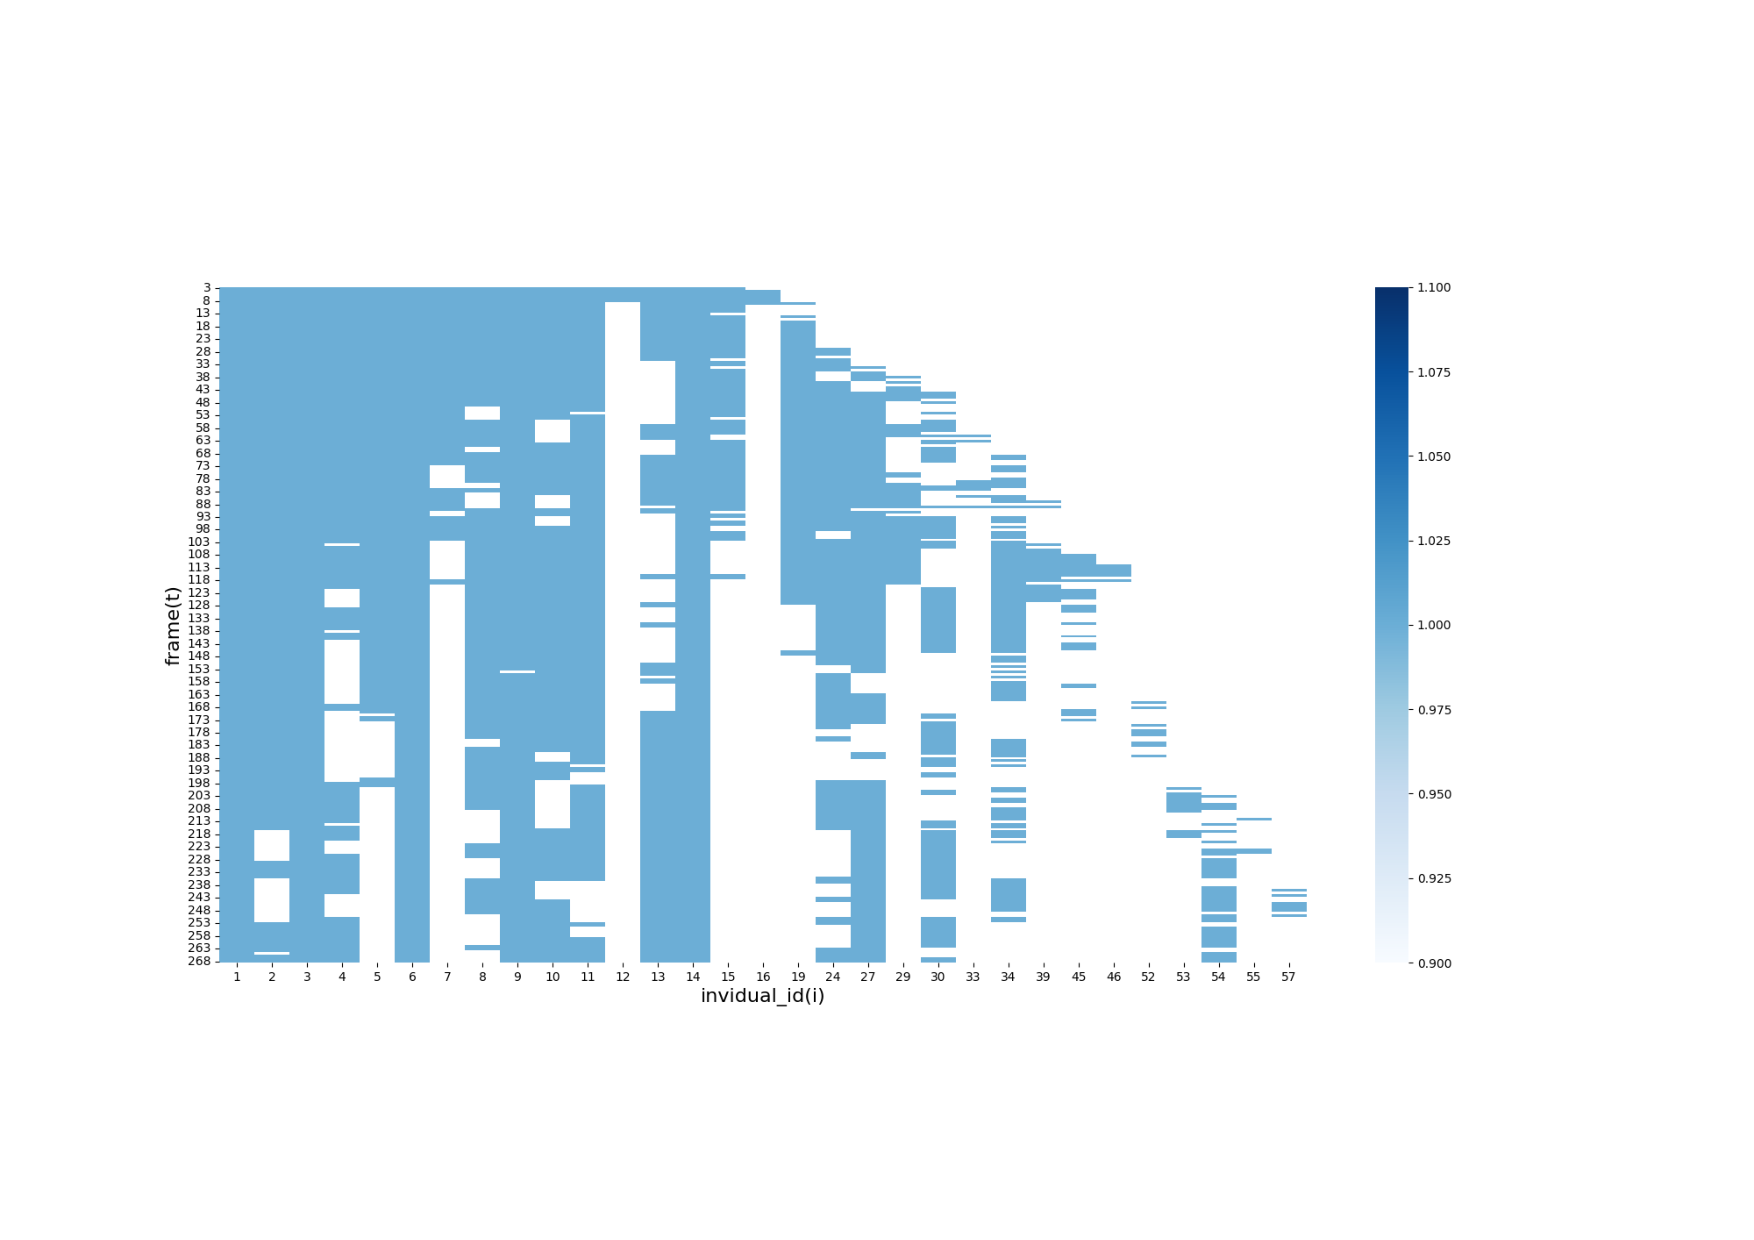
\includegraphics[width=13cm,  keepaspectratio]{existence.pdf}
\caption[Short figure caption for List of Figures]{アリの出現フレーム }
\label{fig:paper1_fig8}
\end{figure}

図4.2(左)では出現回数をID別で可視化しており, IDは出現回数の多い順に左から並べ替えである. 本研究では出現回数75が閾値(75回)と設定してこの閾値以下のアリの追跡データを利用しないことにする. 
\begin{figure}[tbp]
\centering
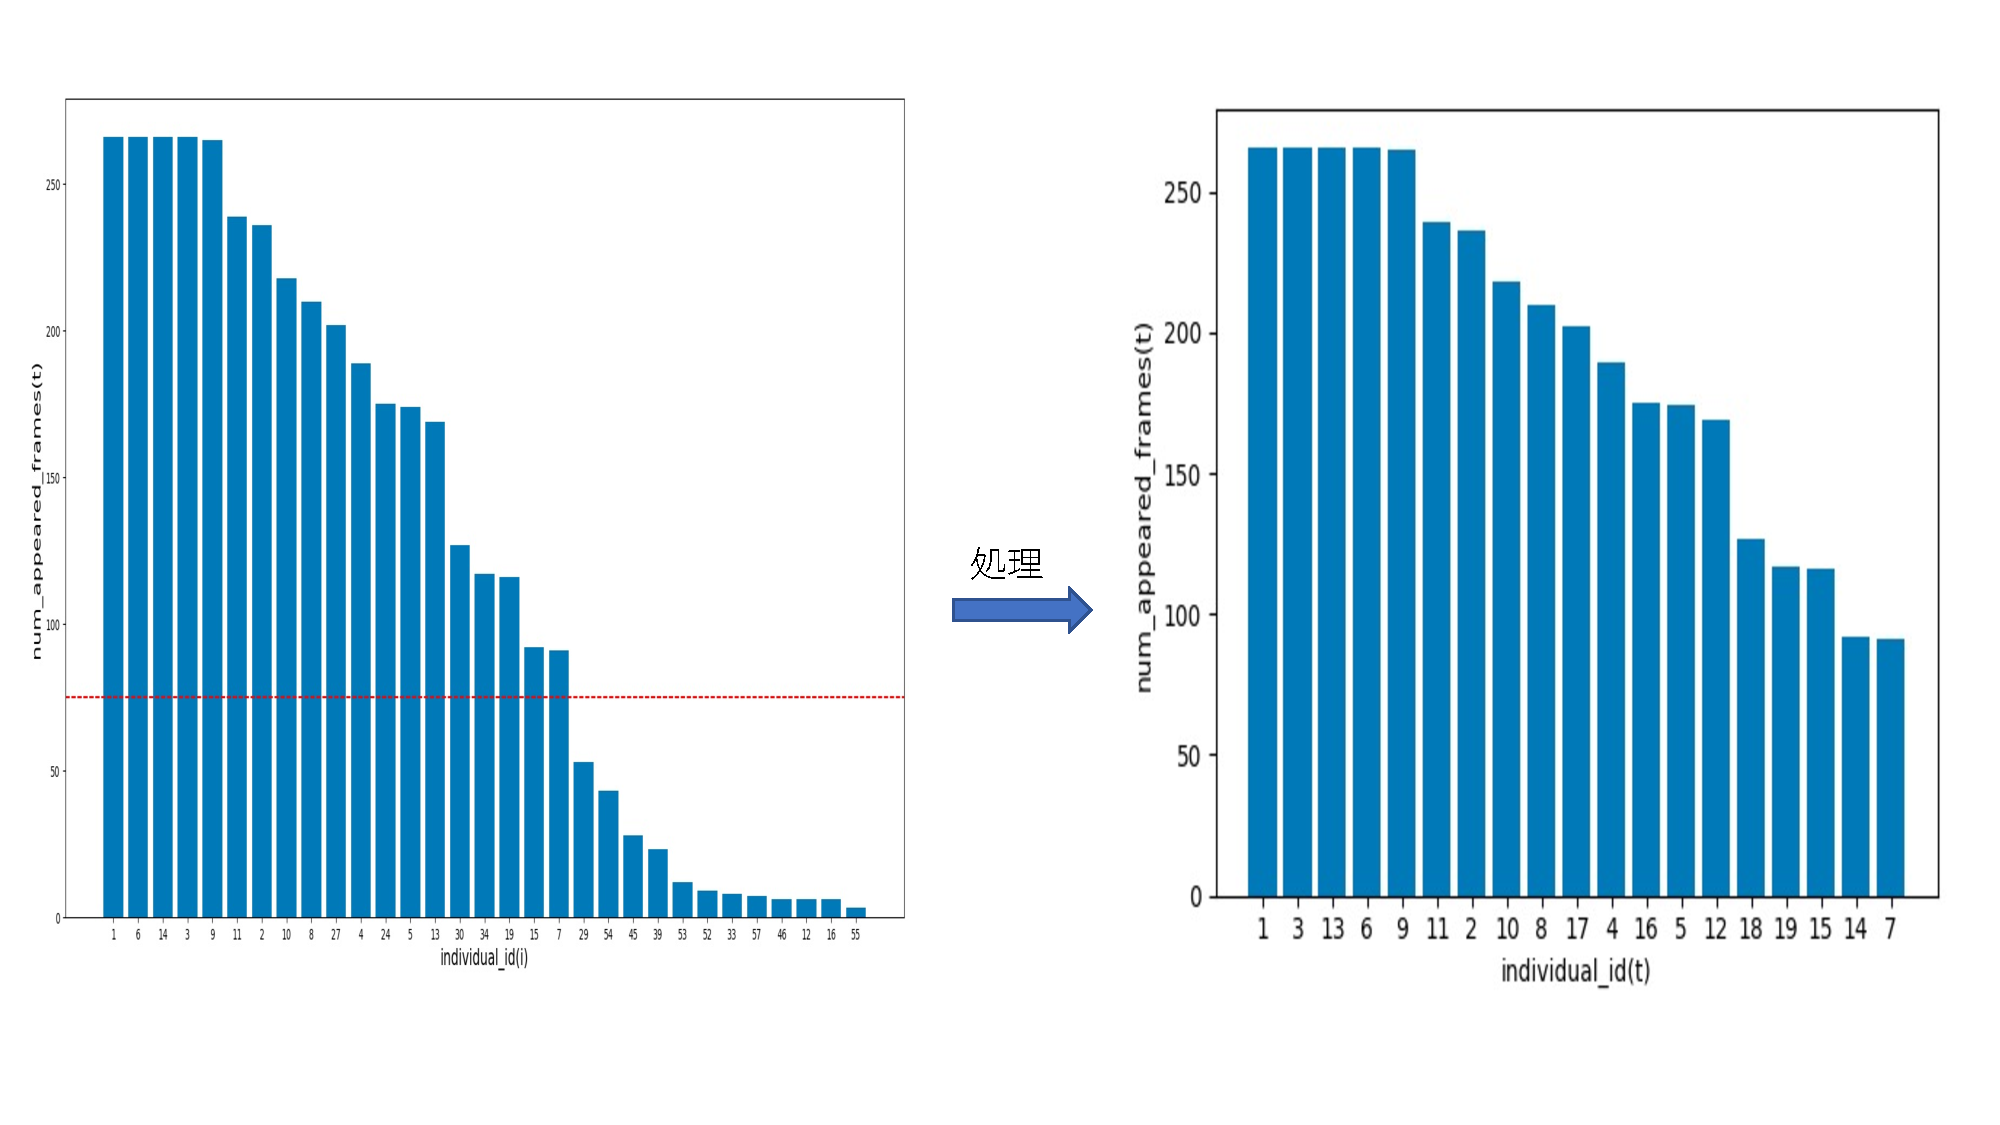
\includegraphics[width=13cm,height=13cm,  keepaspectratio]{existenc.pdf}
\caption[Short figure caption for List of Figures]{アリの出現回数}
\label{fig:paper1_fig9}
\end{figure}
この場合, 閾値を下回った一部の個体ID(図4.2(左)の例では12番など)が欠損することになるので, それ以降の処理では, 欠損したIDが埋まるようにIDを振り直すものとする. IDを振り直した後の, それぞれの個体IDの出現回数を図4.2(右)に示す. 



\section{速度変化の解析}
\label{sec:analys}

まず, それぞれフレームに出現するアリの数を確認する. 図4.3 は各フレーム$t$に出現するアリの数$N_t$を示したものであるが, フレームによって, 追跡されているアリの数が異なることがわかった.
\begin{figure}[tbp]
\centering
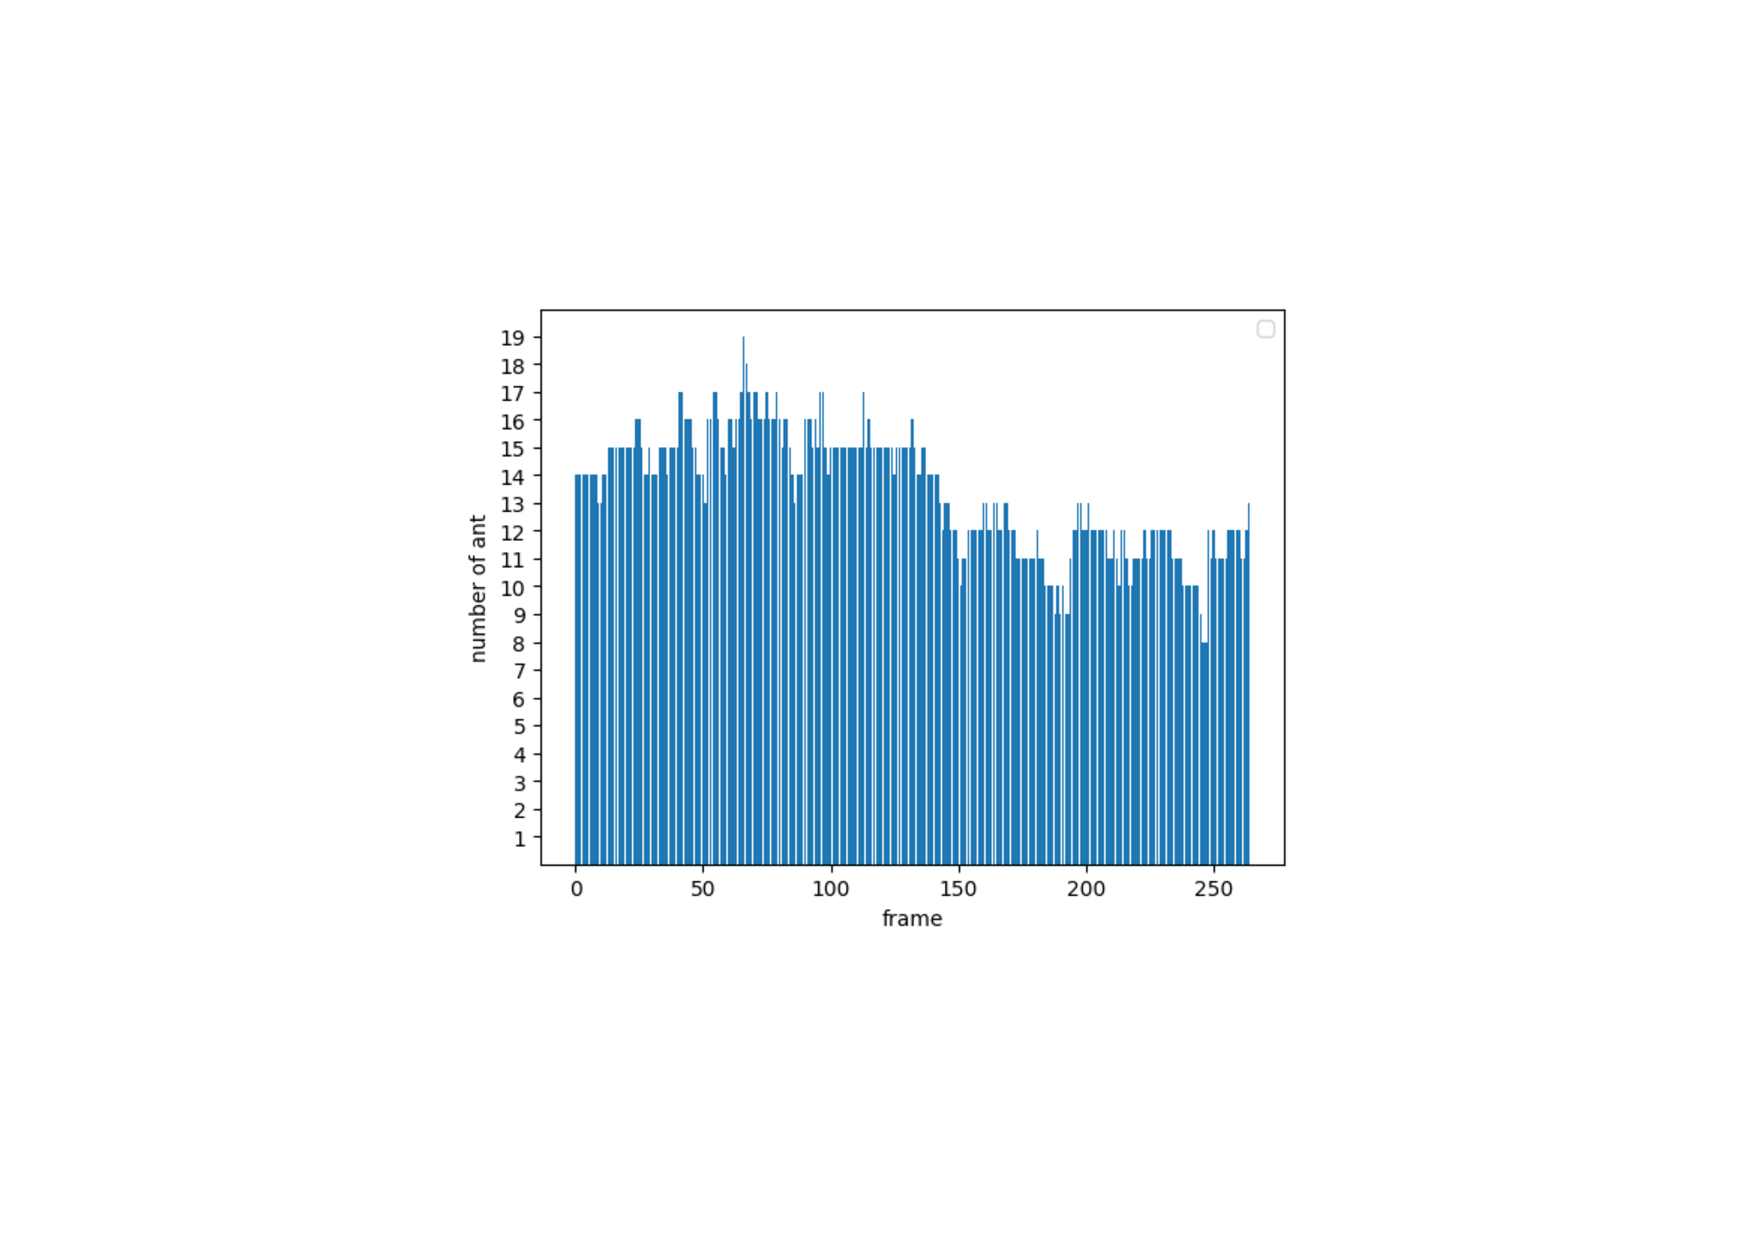
\includegraphics[width=13cm,height = 10cm,  keepaspectratio]{appear.pdf}
\caption[Short figure caption for List of Figures]{各フレームで出現したアリの個体数(横軸はフレーム, 縦軸はそのフレームに出現するアリの個体数)}
\label{fig:paper1_fig10}
\end{figure}
振動刺激提示前後での行動変化を調べるするために速度の解析を行った. アリの速度計算式$\bm{v} = \bm{p}_{t + 1} - \bm{p}_t$を利用して全フレームの全個体の速度を算出する. このとき, 各個体の速度のの大きさ$||v_{i,t}||$の時間変化を図4.4(上)に示す. さらに, フレーム$t$に存在するアリの平均速度$$AvgSpeed_t =\frac{1}{N_t}\sum^{N_t}_{i=1}||\bm{v}_{i,t}|| $$を算出し, その時間変化をプロットしたグラフを図4.4(下)に示す. 

\begin{figure}[tbp]
    \begin{minipage}{0.8\hsize}
        \centering
        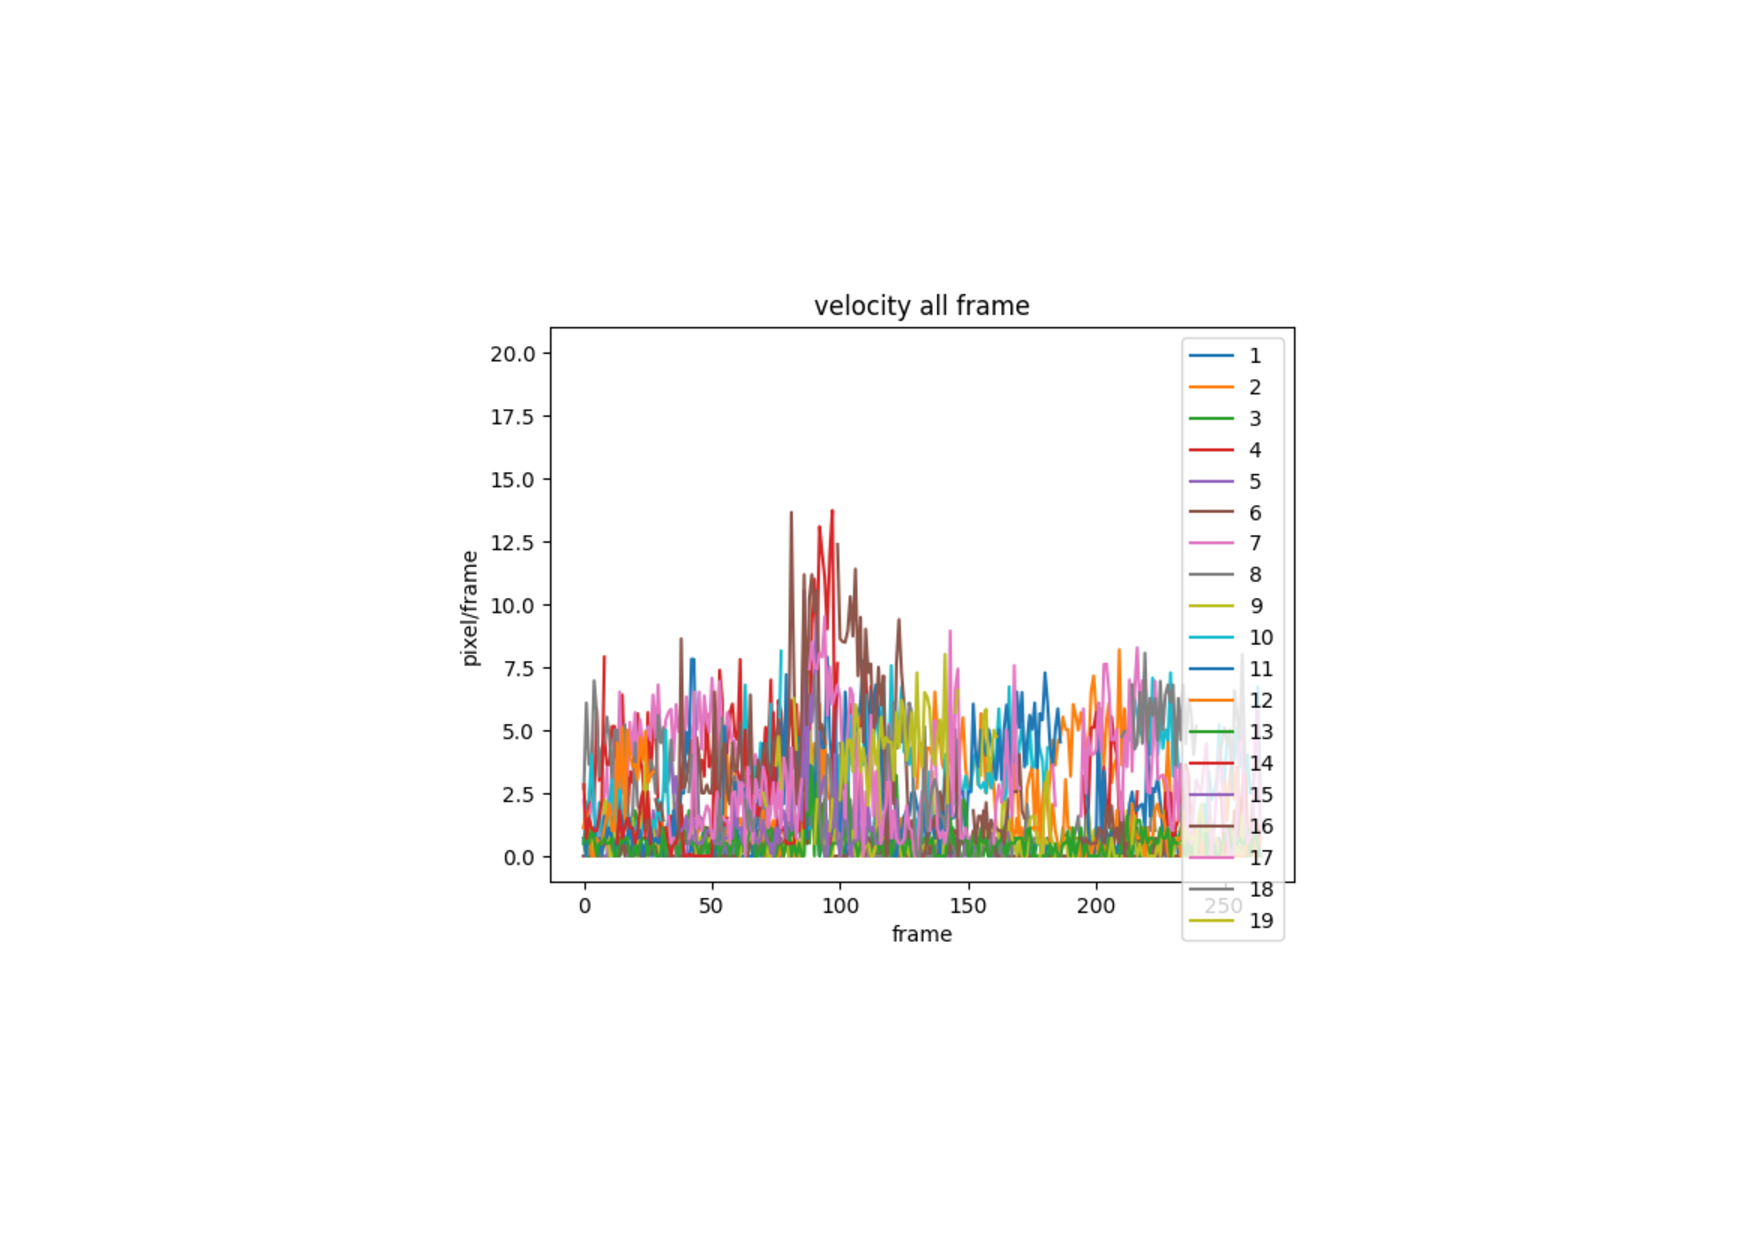
\includegraphics[width=1.3\linewidth]{all_frma.pdf}

        \label{fig:fig11a}
    \end{minipage}
    \begin{minipage}{0.8\hsize}
        \centering
        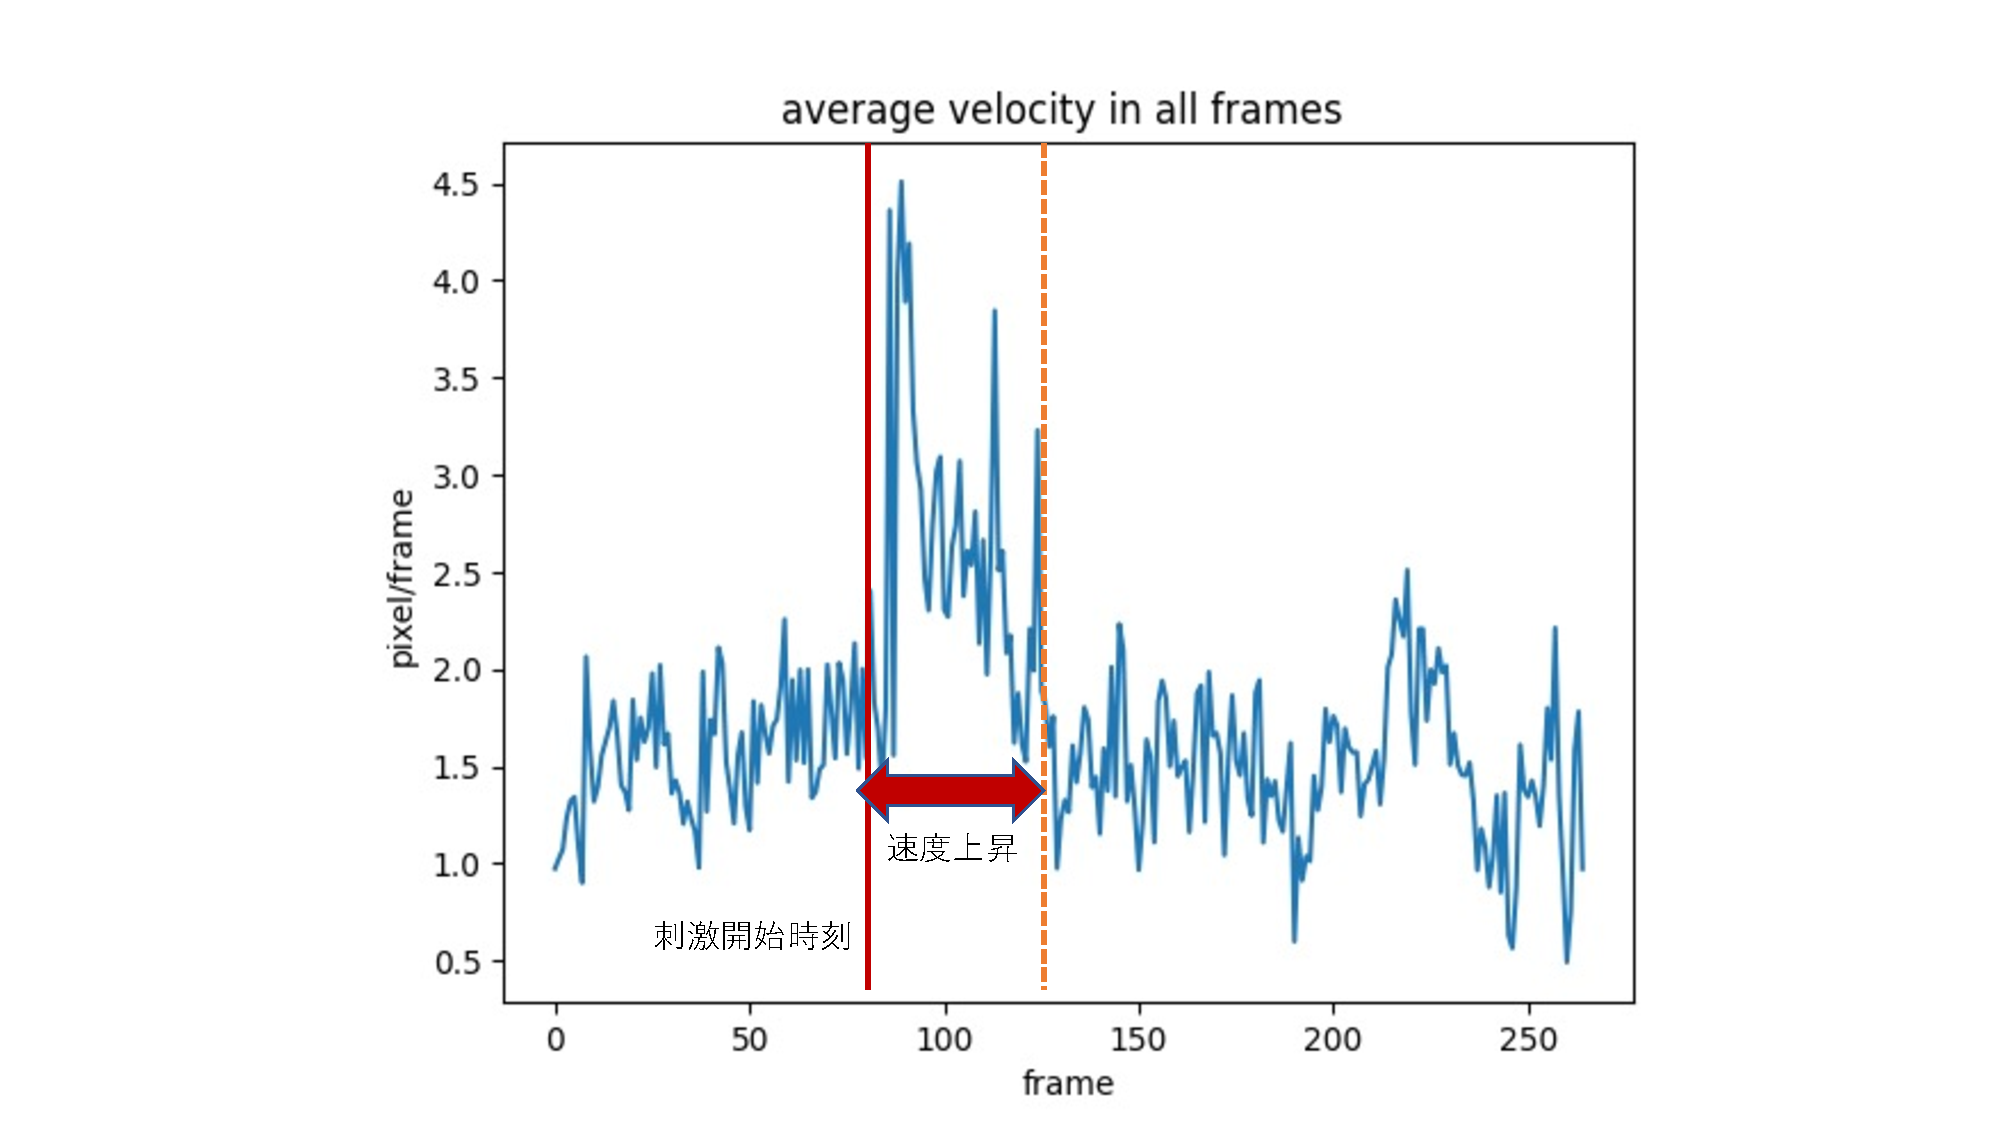
\includegraphics[width=1.3\linewidth]{2.pdf}
       
        \label{fig:fig11b}
    \end{minipage}
    \caption{各個体の速度変化(横軸はフレーム, 縦軸は個々アリの速度(pixel/frame))および全個体の平均速度変化 (横軸はフレーム, 縦軸はそのフレームに出現するアリの平均速度(pixel/frame))}
    \label{fig:fig11}
\end{figure}

図4.4の2つの図を見ると, 刺激を与える時刻(フレーム90)から60フレームの長さ(約2秒間)でアリの速度が上昇したことがわかった. 一番速度が速い時刻は刺激を与えた直後で, その後次第に下がっていき, 最終的に刺激を与える前とほぼ同じ速度となる. 

次に, それぞれの個体の平均速度を解析する. すべてのフレームに出現しないアリがいるため, 全時間帯で平均速度を算出するのではなく, その個体 (ここでは個体$i$とする)の出現フレームの速度の平均を以下の式で算出する. ここで,$T_i$は個体$i$が出現するフレーム番号の集合である. $$AvgSpeed_i =\frac{1}{|T_i|}\sum_{t\in{T_i}}||\bm{v}_{i,t}|| $$

算出した各個体の平均速度を図4.5に示す. この図から刺激を与えられた際によく動いて逃げるアリがいるのに対して, ほとんど影響を受けず逃げないアリが存在することが確認できた. 
\begin{figure}[tbp]
\centering
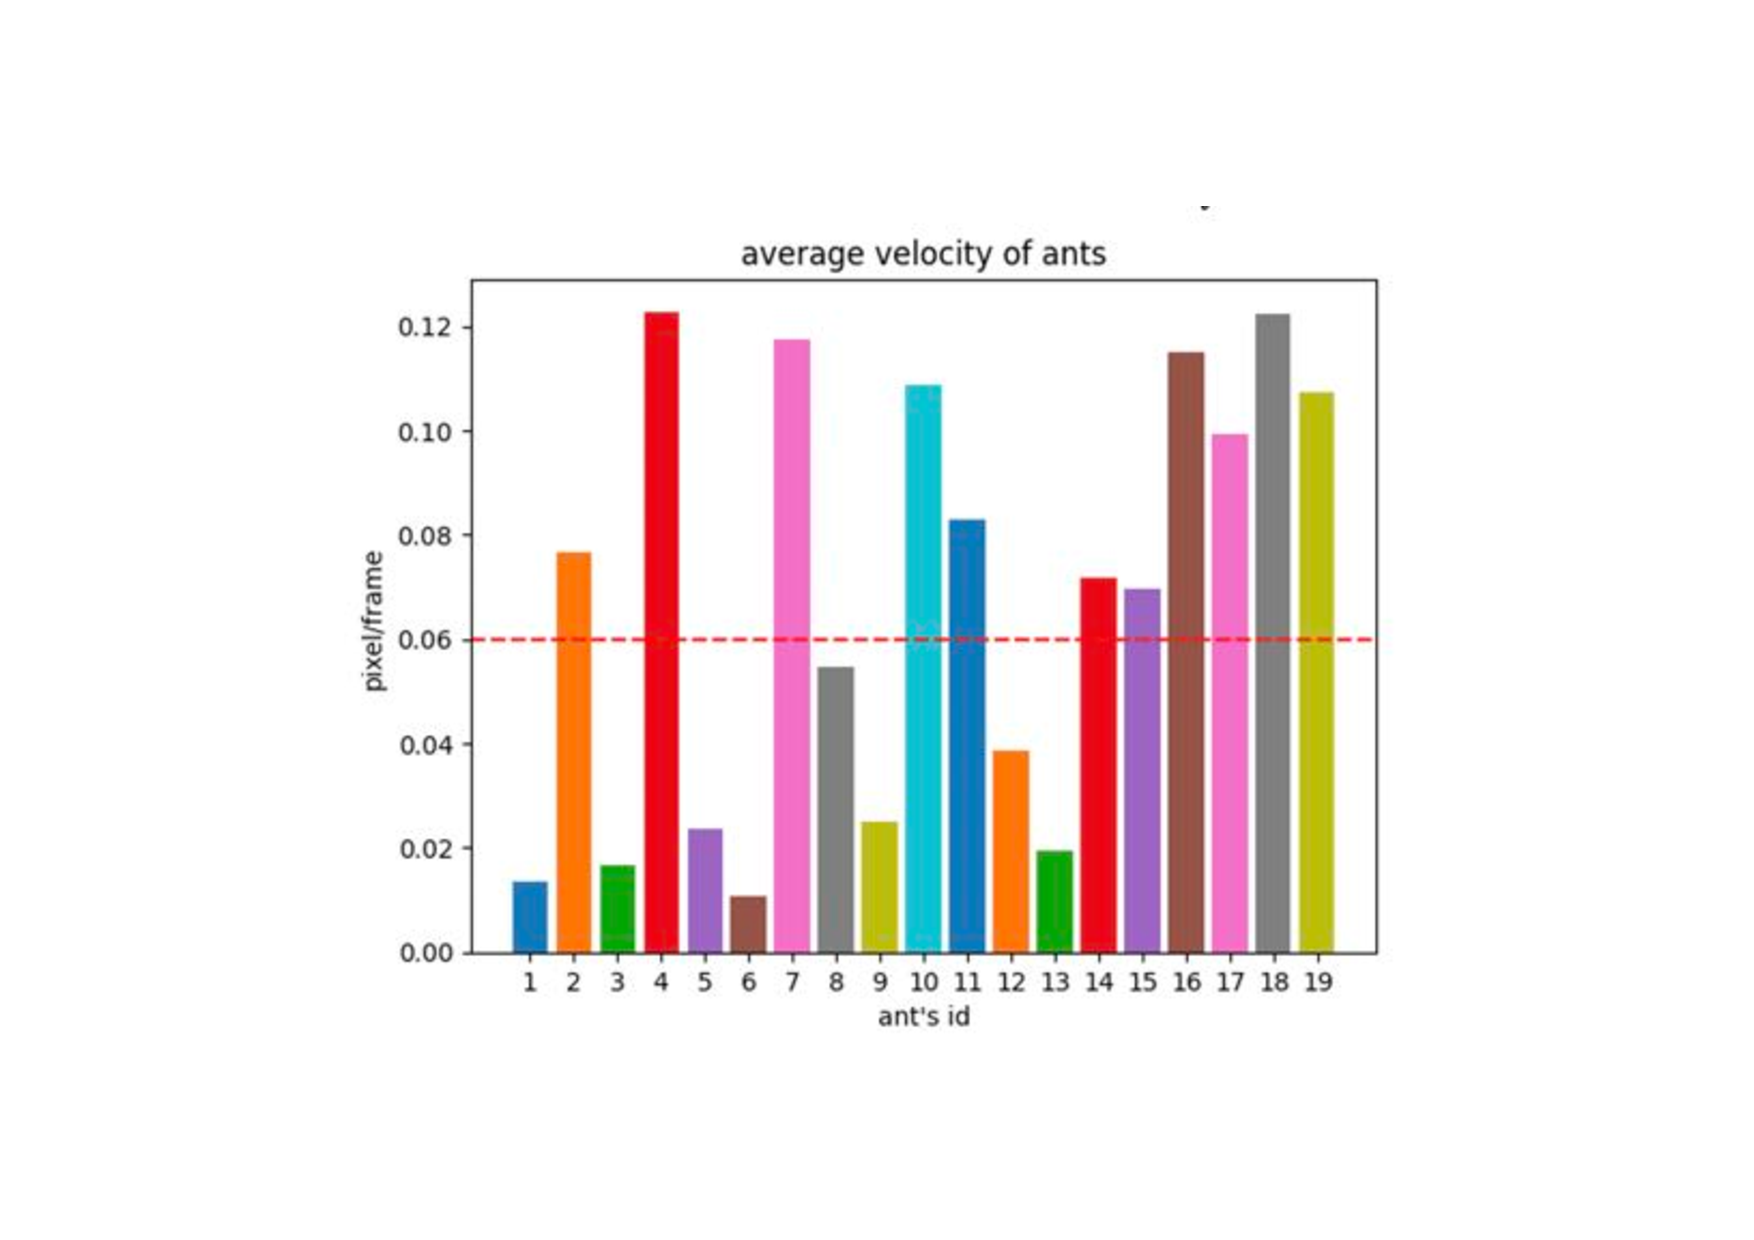
\includegraphics[width=13cm,  keepaspectratio]{kotaivelo.pdf}
\caption[Short figure caption for List of Figures]{個体平均速度 (横軸は個体ID, 縦軸はっ各個体の平均速度 (pixel/frame))}
\label{fig:paper1_fig12}
\end{figure}
同じ刺激を受けてもこのような2つの行動現象が起こる原因を調べるために, 「動かない」と「よく動く」アリにグループを分けてそれぞれの詳細な行動変化を解析する. 
\paragraph{動かないアリ}
比較的動きの小さな個体のうち代表的な個体IDは1,  3,  5,  6,  9,  13である. それぞれのアリの速度変化と位置情報を図4.6に示す. 
\begin{figure}[tbp]
\centering
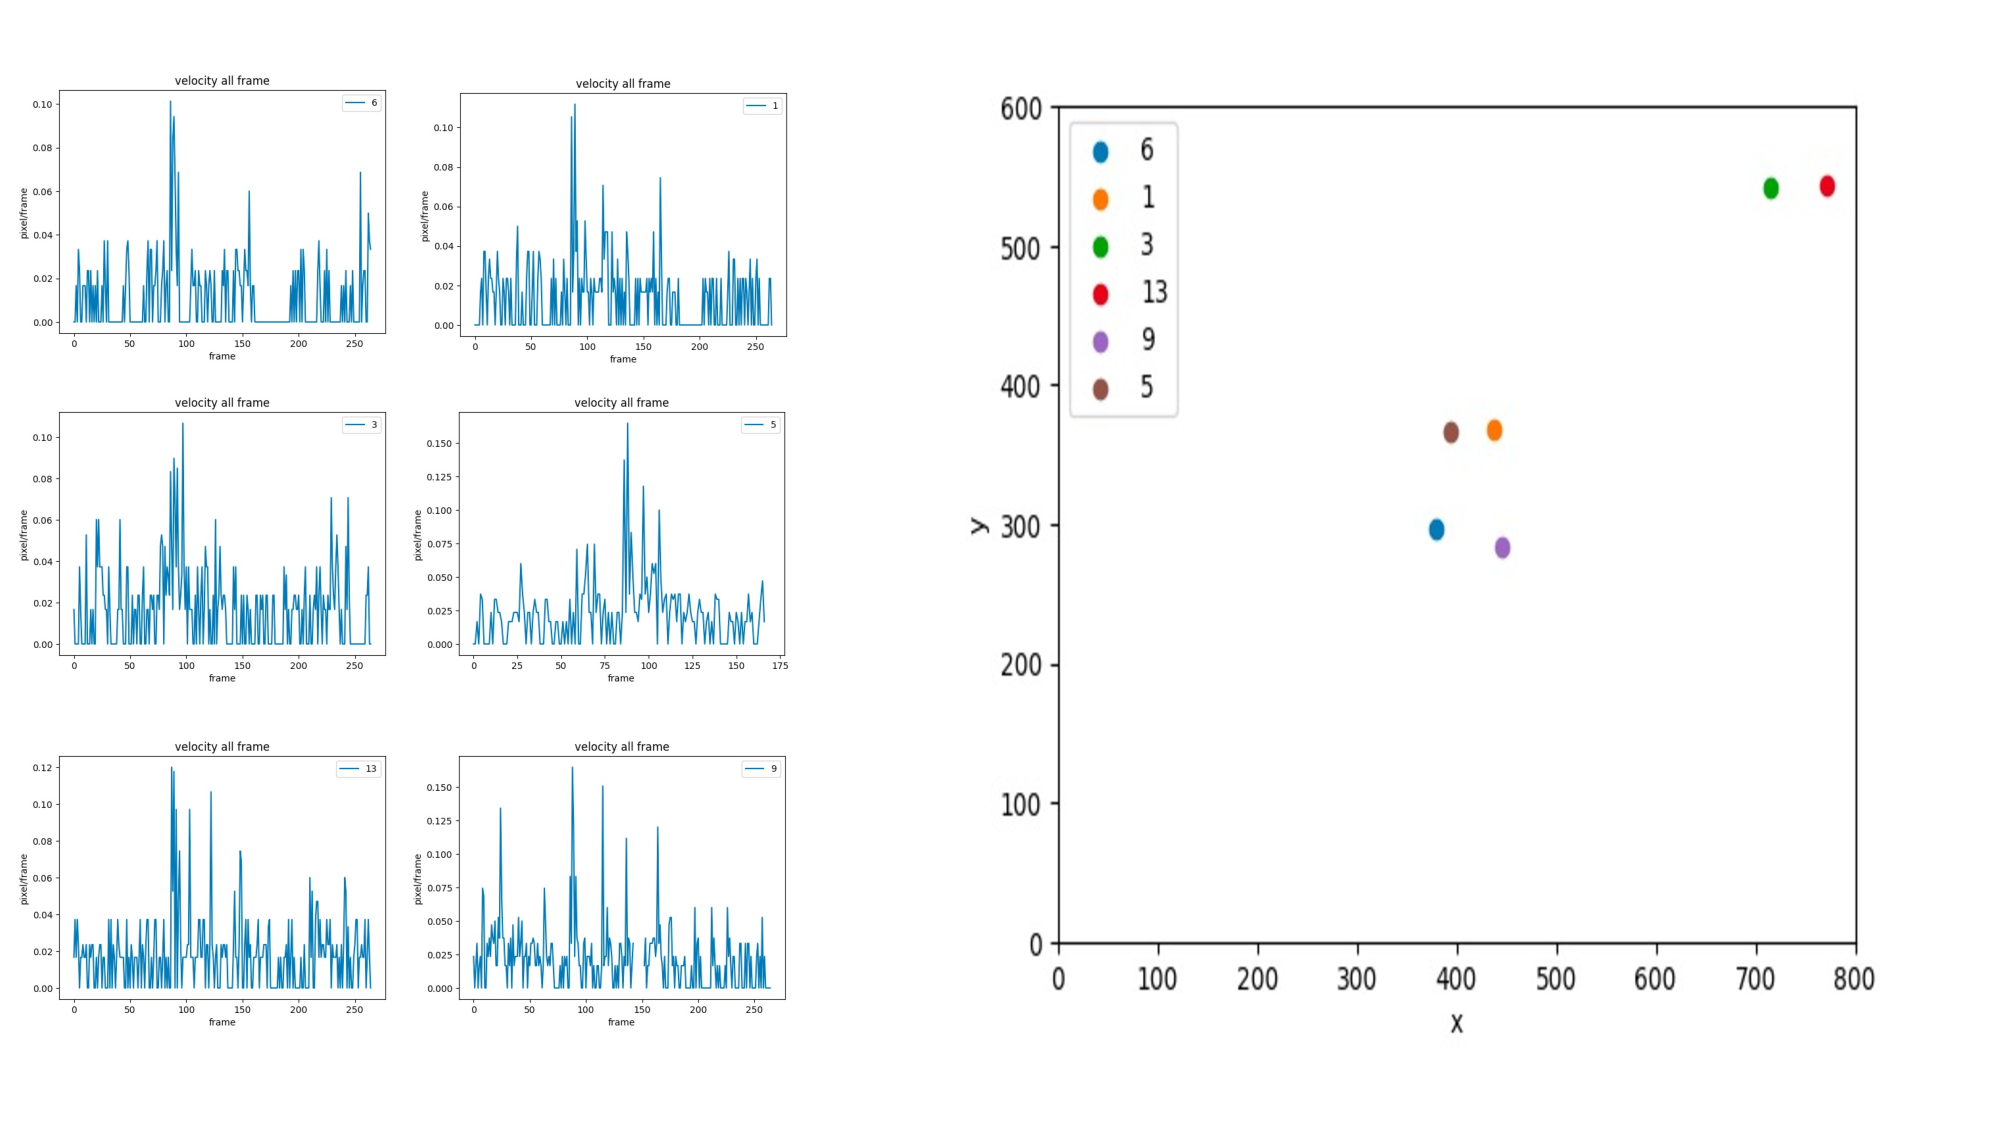
\includegraphics[width=13cm,  keepaspectratio]{nigenai.pdf}
\caption[Short figure caption for List of Figures]{個体速度変化と位置情報}
\label{fig:paper1_fig13}
\end{figure}

まず, それぞれの個体の速度変化を左の図で確認すると, この6匹のアリは刺激を与えられた時刻から速度が上昇したが, 上昇時間は図4.4の全体平均速度上昇時間と比較すると比較的に短いことがわかった. 実際に追跡動画を確認すると6匹の中で実験に動いていない個体はID 1,  3,  6であることがわかった. 刺激時刻の瞬間には速度が上昇しているが, これは実際に用いた板が振動で動いたため,  いずれの個体の位置にも変化が生じて,  大きな速度が算出されたと考えられる. 一方で,  ID 5,  9,  13は刺激時刻直後だけ動いてすぐに止まってしまうことがわかった. 

次に位置情報の図を見ると,  ID 1,  5,  6,  9のアリは実験に用いた板の中心付近にID 3,  13のアリはコロニーの近くにいることがわかった. 中心部にいるアリは餌に執着しており,  コロニーの近くにいるアリはそれ以上逃げる必要性が低いことから, これらのアリは刺激があっても動かないのではないかと考えられる. 

動かないアリのもう1つの特徴はうまく追跡できることである. ID 5のアリは175フレーム, 残りのアリはほとんどのフレームで追跡できている. 
\paragraph{よく動くアリ}
よく動くアリの中から,  平均速度が高くかつ出現フレーム数が多いの個体を選択したところ,  該当する個体のIDは4,  7,  10,  16であった. これらの個体の詳細な軌跡, 速度変化と軌跡(方向を含む)を図4.7と図4.8に示す. 

まず, よく動くアリの速度上昇期間は図4.4の全体平均速度上昇時間と比較するとほとんど同じ傾向が見られる. 
また追跡できるフレームの多いアリを選択したが,動かないアリと比べるとうまく追跡できないことがわかった. 速度が速いアリの方が追跡することが難しいと言える. 
\begin{figure}[tbp]
\centering
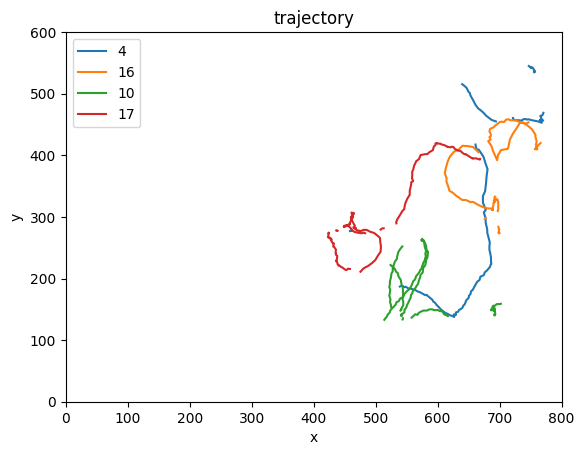
\includegraphics[width=13cm,  keepaspectratio]{traject_nige.png}
\caption[Short figure caption for List of Figures]{逃げるアリの軌跡}
\label{fig:paper1_fig14}
\end{figure}


次に図4.8(右)の移動方向性を見ると, ID4と7のアリの移動方向はコロニー向きである逃げる動きのなっているのに対して, ID 10, 16のアリは中心部に動く傾向が見られる. 
\begin{figure}[tbp]
\centering
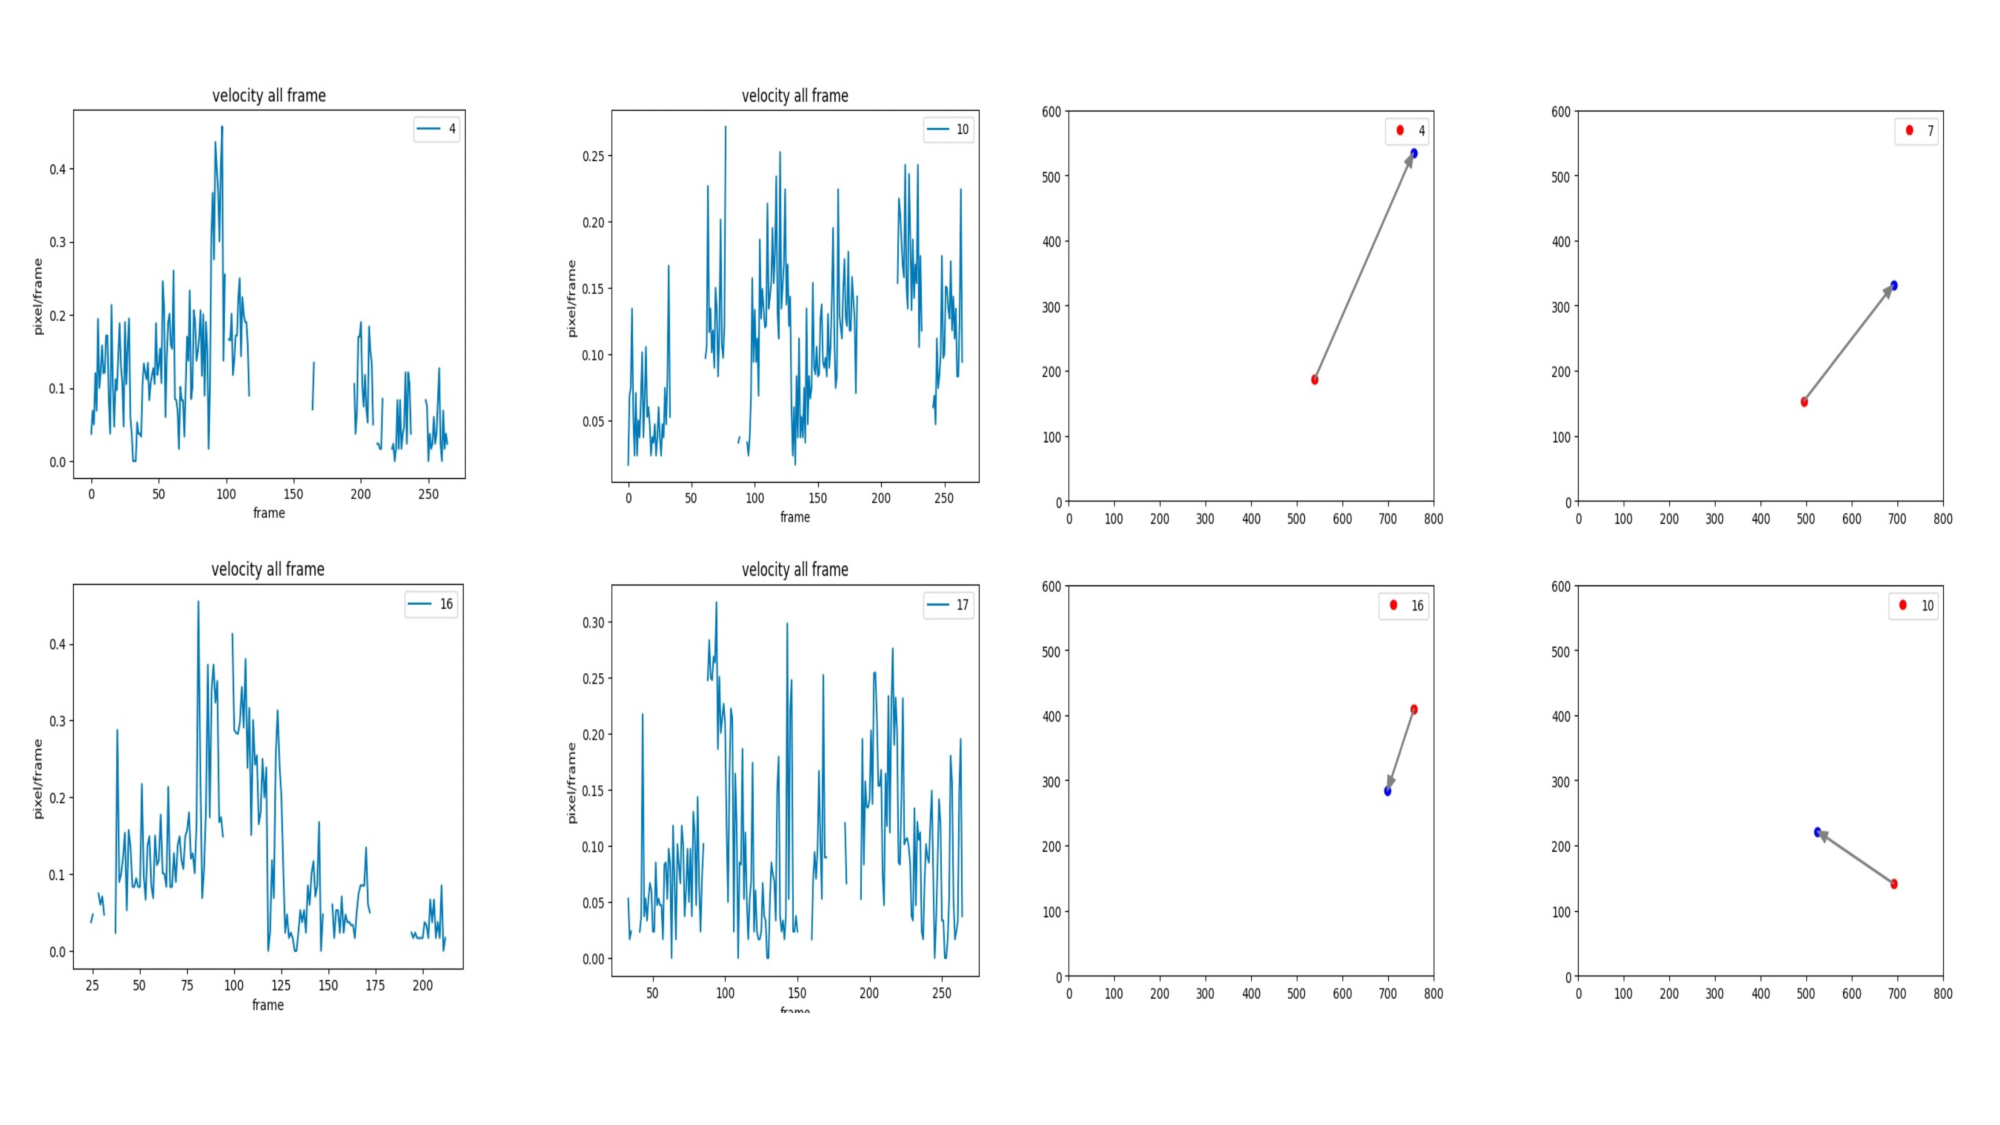
\includegraphics[width=13cm,  keepaspectratio]{velo_hoko_nige.pdf}
\caption[Short figure caption for List of Figures]{逃げるアリの速度と移動方向}
\label{fig:paper1_fig15}
\end{figure}
ID4, 7は最初に中心部の右下のところにいるのに対し10, 16のアリは最初にコロニーのすぐ近くにいる. よく動くアリにおける移動方向の違いは刺激が与えられた際にどの位置にいるか影響されるのではないかと考えられる. 

\section{行動解析より得られた知見}
\label{sec:chiken}
本研究で行った実験を通じて得られた知見を以下にまとめる.
\begin{enumerate}
\item 刺激を与えられるとアリ集団の速度が上昇する傾向が見られるが, 上昇する期間が短くまた元の速度で動く.
\item 同じ刺激を与えられてもすぐに逃げていくアリと逃げないアリがいる.
\item 逃げないアリの方は速度上昇期間は短かく, 実験に用いた板の中心部(餌の近辺), またはコロニーの近くにいることが多い.
\item 逃げていくアリの方は速度上昇期間が長く, 移動軌跡としてはコロニーに戻る傾向が見られる.
\end{enumerate}


%%




\renewcommand{\arraystretch}{2}  % make spacing nicer


\chapter{結論}
本研究では振動刺激によるアリの行動変化を実験を通じて得られた動画を用いて解析した. 本研究で実施した実験方法には問題が存在するのと追跡手法の限界があるため十分精度を持つ手法ではないが, 振動刺激を与えた際の動画解析から,  アリの移動軌跡を解析することで,  振動前後のアリの行動変化を解析すること,  および個々の個体を解析できることが示された. したがって,  本研究で行った解析の枠組みを発展させることで,  アリの行動研究に貢献できると考えられる. 

本研究では扱えなかった点, および今後の課題を以下にまとめる. 
\paragraph{実験方法}振動刺激を与える時,  中心部のアリは端のアリと比べて振動を受ける力が小さい. その結果は中心部のアリの方があまり動かないことにつながったと考えられるが, それぞれのアリの行動変化の違いを調べるために均等に刺激を与える必要がある. 

また本研究の実験ではアリの数が変化ことによりアリの数が多すぎる状況では個体同士の重なりなどの原因でうまく追跡できないケースがあった. 追跡をうまく行うために,  実験時からアリの数を抑えることができるような実験方法を考案する必要がある. 

\paragraph{アリの生息環境の考慮}
本研究では研究室内と野外の両方の実験動画を定性的に比較することができた. その結果,  研究室内と比較すると, 野外アリの方が刺激に対して敏感であることに気づいた. 本研究では,  野外実験は振動刺激の与え方の点で解析が困難であると判断したが,  野外実験がうまくできれば研究室内と野外のアリの行動比較などもできて,  生息環境がアリの行動にどのように影響するかを確認できると考えられる. 
\paragraph{追跡手法}本研究ではYOLOv5とStrongSORTでアリの動画を追跡したが, 十分な精度は確保できておらず,  正確な解析には追跡結果の修正が必要であることがわかった. これは,  これらの手法ではアリの見た目の特徴に強く依存するために,  見た目が類似し,  かつ動きが速いアリの追跡には限界があると考えらる. 今後,  アリの動画追跡手法を考慮する必要がある. 
\paragraph{相互作用解析}アリは集団で暮らしているので個体間で互いに影響しあっている. 1匹の動きは他の個体にどのぐらい影響するか,  個体間の相互作用を解析することで,  よりアリの行動の研究に貢献できると考えられる. 

\chapter*{謝辞}

川嶋宏彰教授には本研究に関して様々な助言をしていただきました. 深く感謝致します. 

明治大学・西森研究室の西森拓教授・白石允梓准教授・久本峻平研究員には毎回のミーティングで助言していただき, そして久本峻平研究員には実験方法を教えて際に実験を行っていただき深く感謝致します. 

また川嶋研究室の皆様には日頃から様々な形でお世話になり大変感謝してこの場を借りてお礼申し上げます. 
% 参考文献
% {
% \footnotesize
\bibliographystyle{junsrt}
\bibliography{sotsuronhoangbahung}

% }


\end{document}
